\documentclass[11pt,a4paper]{article}
\usepackage[margin=2.4cm]{geometry}
% ---------------------------------------------------------------
%  Shared preamble: notation, colours, listings, theorem envs
% ---------------------------------------------------------------
\usepackage[T1]{fontenc}
\usepackage[utf8]{inputenc}
\usepackage{lmodern}
\usepackage{amsmath,amssymb,amsthm}
\usepackage{mathtools}
\usepackage{booktabs}
\usepackage{tabularx}
\usepackage{array}
\usepackage{multirow}
\usepackage{graphicx}
\usepackage{xcolor}
\usepackage{listings}
\usepackage{tikz}
\usetikzlibrary{arrows.meta,positioning,fit,backgrounds,calc,shapes.geometric,decorations.pathreplacing}
\usepackage{caption}

% ---------- palette (colour-blind safe, prints legibly in grey) ----------
\definecolor{cBlue}{HTML}{2B6CB0}
\definecolor{cBlueBg}{HTML}{E7F0FB}
\definecolor{cAmber}{HTML}{B4690E}
\definecolor{cAmberBg}{HTML}{FDF0D5}
\definecolor{cGreen}{HTML}{2F855A}
\definecolor{cGreenBg}{HTML}{E8F5EC}
\definecolor{cPurple}{HTML}{7B3FA0}
\definecolor{cPurpleBg}{HTML}{F6ECFA}
\definecolor{cGrey}{HTML}{6B6B76}
\definecolor{cGreyBg}{HTML}{F1F1F4}
\definecolor{cRed}{HTML}{B03030}
\definecolor{cInk}{HTML}{1A1A1E}

% ---------- U-semiring / Q-expression notation ----------
\newcommand{\Usemi}{\ensuremath{\mathcal{U}}}
\newcommand{\Nbar}{\ensuremath{\overline{\mathbb{N}}}}
\newcommand{\sq}[1]{\ensuremath{\left\lVert #1 \right\rVert}}       % squash
\newcommand{\notu}[1]{\ensuremath{\mathrm{not}(#1)}}                % negation
\newcommand{\ind}[1]{\ensuremath{[\,#1\,]}}                          % indicator
\newcommand{\usum}[1]{\ensuremath{\sum_{#1}}}                        % unbounded sum
\newcommand{\den}[1]{\ensuremath{[\![ #1 ]\!]}}                      % denotation
\newcommand{\Tup}[1]{\ensuremath{\mathrm{Tuple}(#1)}}
\newcommand{\Sumagg}{\ensuremath{\mathrm{Sum}}}
\newcommand{\lam}[2]{\ensuremath{\lambda #1.\,#2}}
\newcommand{\qop}{\ensuremath{\mathrm{QOp}}}
\newcommand{\hop}{\ensuremath{\mathrm{HOp}}}
\newcommand{\zzero}{\ensuremath{\mathbf{0}}}
\newcommand{\oone}{\ensuremath{\mathbf{1}}}

% ---------- inline tags ----------
\newcommand{\udp}{\textsc{UDP}}
\newcommand{\QED}{\textsc{Qed}}
\newcommand{\sqlsolver}{\textsc{SQLSolver}}
\newcommand{\spes}{\textsc{SPES}}
\newcommand{\wetune}{\textsc{WeTune}}
\newcommand{\lia}{\textsf{LIA}}
\newcommand{\liastar}{\textsf{LIA}\ensuremath{^*}}

% ---------- code listings ----------
\lstdefinestyle{sql}{
  language=SQL,
  basicstyle=\ttfamily\small\color{cInk},
  keywordstyle=\color{cBlue}\bfseries,
  commentstyle=\color{cGrey}\itshape,
  stringstyle=\color{cGreen},
  showstringspaces=false,
  breaklines=true,
  columns=fullflexible,
  keepspaces=true,
  morekeywords={ALL,DISTINCT,GROUP,BY,ORDER,INTERSECT,EXCEPT,VALUES,OVER,PARTITION}
}
\lstdefinestyle{plan}{
  basicstyle=\ttfamily\footnotesize\color{cInk},
  breaklines=false,
  columns=fullflexible,
  keepspaces=true,
  escapeinside={(@}{@)}
}
\lstdefinestyle{pseudo}{
  basicstyle=\ttfamily\small\color{cInk},
  keywordstyle=\color{cPurple}\bfseries,
  morekeywords={procedure,function,for,all,if,then,else,return,while,do,end,foreach,and,or,not},
  breaklines=true,
  columns=fullflexible,
  keepspaces=true,
  mathescape=true
}
\lstset{style=sql}

% ---------- boxed "key idea" ----------
\newcommand{\keybox}[2]{%
  \begin{center}
  \begin{tikzpicture}
    \node[draw=cAmber,fill=cAmberBg,line width=0.9pt,rounded corners=3pt,
          inner sep=8pt,text width=0.92\linewidth,align=left]
      {\textbf{\color{cAmber}#1}\\[2pt]#2};
  \end{tikzpicture}
  \end{center}}

\newcommand{\warnbox}[2]{%
  \begin{center}
  \begin{tikzpicture}
    \node[draw=cRed,fill=cGreyBg,line width=0.9pt,rounded corners=3pt,
          inner sep=8pt,text width=0.92\linewidth,align=left]
      {\textbf{\color{cRed}#1}\\[2pt]#2};
  \end{tikzpicture}
  \end{center}}

\usepackage[colorlinks=true,linkcolor=cBlue,citecolor=cGreen,urlcolor=cBlue]{hyperref}

\theoremstyle{definition}
\newtheorem{definition}{Definition}[section]
\newtheorem{example}[definition]{Example}
\theoremstyle{plain}
\newtheorem{theorem}[definition]{Theorem}
\newtheorem{lemma}[definition]{Lemma}
\theoremstyle{remark}
\newtheorem{remark}[definition]{Remark}

\title{\bfseries Proving SQL Queries Equivalent\\[4pt]
\large U-expressions, Q-expressions, and \liastar{}\\[6pt]
\normalsize A from-scratch guide for people who want to \emph{implement} these algorithms}
\author{}
\date{}

\begin{document}
\maketitle
\thispagestyle{empty}

\begin{abstract}
\noindent
Three systems dominate automated SQL equivalence checking under bag semantics:
\udp{} (Chu et al., VLDB 2018), which introduced \emph{U-expressions} and the U-semiring;
\QED{} (Wang, Pan and Cheung, VLDB 2024), which redesigned them into \emph{Q-expressions}; and
\sqlsolver{} (Ding et al., SIGMOD 2024), which kept U-expressions and replaced the
decision procedure with the theory \liastar{}.
This document explains all three from first principles. We assume you know SQL and
nothing else --- no semiring theory, no SMT, no proof assistants.
Every symbol is introduced with a SQL query that exhibits it, every algorithm is given
as pseudocode you could type in, and every claim about the three systems is traced to a
specific definition, theorem or table in the source papers.
Plans are shown as Apache Calcite \texttt{RelNode} trees (the representation all three
systems actually consume) with PostgreSQL plans as a secondary, executable cross-check.
\end{abstract}

\vspace{4pt}
\noindent\textbf{How to read this.}
Section~\ref{sec:prelim} builds the counting-function view of SQL and fixes a running
example. Section~\ref{sec:uexpr} is U-expressions end to end. Section~\ref{sec:qexpr} is
Q-expressions end to end. Section~\ref{sec:lia} is \liastar{}. Section~\ref{sec:compare}
compares the three on examples chosen to separate them. Section~\ref{sec:impl} is an
implementer's checklist. Appendix~\ref{app:axioms} collects every axiom on one page.

\tableofcontents
\newpage

\section{The problem, and why it is hard}
\label{sec:intro}

\subsection{What we are trying to decide}

Given two SQL queries $Q_1$ and $Q_2$ over the same schema, decide whether they return
the same answer \emph{on every possible database instance}. Not on your data --- on all data.

This matters because every relational engine contains a rule-based rewriter. Calcite,
Spark SQL, CockroachDB and PostgreSQL all transform your query into a different one before
executing it. If a rewrite rule is wrong, the engine silently returns wrong answers.
Historically these bugs have been found by users, years later~\cite{udp}.

The general problem is undecidable. For queries with negation and arbitrary predicates you
can encode first-order validity, so no algorithm decides all cases. Everything in this
document is therefore a \emph{sound but incomplete} procedure: when it says
``equivalent'' it is right; when it says ``unknown'' the queries may still be equivalent.

\keybox{The three answers a prover may give}{%
\textbf{EQUIVALENT} --- proved, trust it.\quad
\textbf{NOT EQUIVALENT} --- a counterexample database exists.\quad
\textbf{UNKNOWN} --- the procedure ran out of power.
\\[3pt]
All three systems here answer EQUIVALENT or UNKNOWN. None of them is a
counterexample finder. Refutation is a different problem, usually attacked
by bounded model finding.}

\subsection{Bag semantics, and why it changes everything}

SQL tables are \emph{bags} (multisets): duplicates are real and observable.
\lstinline|SELECT x FROM R| does not deduplicate. Two queries that agree as sets may
disagree as bags:

\begin{lstlisting}[style=sql]
SELECT x FROM R                 -- may return 1, 1, 2
SELECT DISTINCT x FROM R        -- returns    1, 2
\end{lstlisting}

The classical theory of query equivalence (containment mappings, the chase, homomorphism
checking) is set-based. Under bags the picture is harder: bag \emph{containment} of
conjunctive queries is a long-standing open problem, while bag \emph{equivalence} of unions
of conjunctive queries is decidable~\cite{cohen}. That decidability result is the
theoretical anchor for all three systems.

\subsection{The common architecture}

All three systems share a pipeline:

\begin{center}
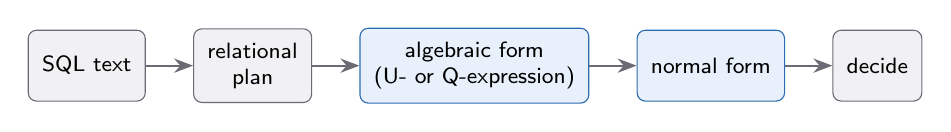
\begin{tikzpicture}[node distance=6mm,
  box/.style={draw=cGrey,fill=cGreyBg,rounded corners=3pt,inner sep=5pt,
              font=\footnotesize\sffamily,minimum height=9mm,align=center},
  hi/.style ={draw=cBlue,fill=cBlueBg,rounded corners=3pt,inner sep=5pt,
              font=\footnotesize\sffamily,minimum height=9mm,align=center},
  ar/.style ={-{Stealth[length=2.4mm]},cGrey,thick}]
\node[box] (sql) {SQL text};
\node[box,right=of sql] (plan) {relational\\plan};
\node[hi,right=of plan]  (alg) {algebraic form\\(U- or Q-expression)};
\node[hi,right=of alg]  (norm) {normal form};
\node[box,right=of norm] (dec) {decide};
\draw[ar] (sql)--(plan); \draw[ar] (plan)--(alg);
\draw[ar] (alg)--(norm); \draw[ar] (norm)--(dec);
\end{tikzpicture}
\end{center}

They differ in exactly two places, and it is worth stating this up front because everything
else follows from it:

\begin{enumerate}
\item \textbf{The algebraic form.} \udp{} and \sqlsolver{} use \emph{U-expressions},
      defined \emph{axiomatically} over an abstract structure called a U-semiring.
      \QED{} uses \emph{Q-expressions}, which are the same syntax pinned to a
      \emph{concrete} semantic domain $\Nbar = \mathbb{N}\cup\{\infty\}$.
\item \textbf{The decision step.} \udp{} compares normal forms \emph{syntactically}.
      \QED{} encodes them into first-order logic and calls an SMT solver.
      \sqlsolver{} encodes them into \liastar{}, a theory built for unbounded sums, and
      reduces that to plain \lia{} for an SMT solver.
\end{enumerate}

\begin{table}[h]
\centering\small
\begin{tabularx}{\linewidth}{@{}l l l X@{}}
\toprule
 & \textbf{algebra} & \textbf{decision step} & \textbf{one-line character} \\
\midrule
\udp{} 2018      & U-expression & syntactic isomorphism & the foundation; proves things by axiom-chasing \\
\QED{} 2024      & Q-expression & SMT on FOL encoding   & better \emph{modelling}: NULLs, constraints, unknown operators \\
\sqlsolver{} 2024& U-expression & \liastar{} $\to$ \lia{} $\to$ SMT & better \emph{arithmetic}: unbounded sums, real aggregates \\
\bottomrule
\end{tabularx}
\caption{The three systems at a glance. \spes{}~\cite{spes}, a fourth system, uses a
\emph{tree-structured} algebraic representation of relational operators rather than a
U-expression, normalises it with hand-written rewrite rules, and calls an SMT solver only to
compare predicates; we use it as a baseline throughout.}
\end{table}

\subsection{A warning about the published numbers}

Every paper reports how many query pairs it proves on ``the Calcite test suite''. These
numbers are \emph{not} comparable across papers, because each group extracted its own pairs
from a different Calcite version with a different filter. The clearest evidence: \QED{} and
\sqlsolver{} both report \spes{} on ``232 Calcite pairs'' and get \textbf{95} and
\textbf{99} respectively. Treat cross-paper percentages as indicative only. We return to
this in Section~\ref{sec:compare}.

\section{Preliminaries: a table is a counting function}
\label{sec:prelim}

\subsection{The one idea everything rests on}

Write a bag not as a list of rows but as a function that counts:

\keybox{Definition you must internalise}{%
$R(t)$ = ``how many copies of the row $t$ are in table $R$?''\\[3pt]
A table of schema $\sigma$ is a function $\Tup{\sigma} \to \mathbb{N}$, where
$\Tup{\sigma}$ is the set of \emph{all} tuples of that schema --- not just the ones
present. Absent rows simply have count $0$.}

This is the \emph{$K$-relation} view of Green, Karvounarakis and Tannen~\cite{green}, with
$K = \mathbb{N}$. Running example throughout:

\begin{center}\small
\begin{tabular}{@{}ll@{}}
\begin{tabular}{@{}c|c@{}}
\multicolumn{2}{@{}l}{$R$}\\
\toprule
$x$ & $y$\\\midrule
1 & 10\\ 1 & 20\\ 2 & 30\\\bottomrule
\end{tabular}
&\hspace{12mm}
\begin{tabular}{@{}c|c@{}}
\multicolumn{2}{@{}l}{$S$ \small(primary key on $a$)}\\
\toprule
$a$ & $b$\\\midrule
1 & 100\\\bottomrule
\end{tabular}
\end{tabular}
\end{center}

\noindent so $R(1,10)=1$, $R(1,20)=1$, $R(2,30)=1$, and $R(t)=0$ for every other $t$;
$S(1,100)=1$ and $S(t)=0$ elsewhere. Verified:

\begin{lstlisting}[style=sql]
select count(*) from r where x = 1 and y = 10;   --> 1
select count(*) from r where x = 1 and y = 99;   --> 0
\end{lstlisting}

\subsection{Query operators as arithmetic}

Once tables are counting functions, the relational operators become arithmetic. This table
is the Rosetta stone for the whole document; each line is derived properly in
Section~\ref{sec:uexpr}.

\begin{table}[h]\centering\small
\begin{tabularx}{\linewidth}{@{}l l X@{}}
\toprule
\textbf{SQL} & \textbf{on counts} & \textbf{why} \\
\midrule
\lstinline|FROM R|                & $R(t)$ & by definition \\
\lstinline|WHERE b|               & $\ind{b}\times R(t)$ & $\ind{b}$ is $1$ or $0$; multiplying by $0$ deletes the row \\
\lstinline|R, S| (cross join)     & $R(t_1)\times S(t_2)$ & every left row pairs with every right row \\
\lstinline|UNION ALL|             & $R(t)+S(t)$ & copies accumulate \\
\lstinline|SELECT x| (projection) & $\usum{y} R(x,y)$ & forgetting $y$ merges rows, so counts add \\
\lstinline|DISTINCT|              & $\sq{R(t)}$ & clamp any count to $0$ or $1$ \\
\lstinline|NOT EXISTS Q|          & $\notu{\usum{t}Q(t)}$ & $1$ exactly when the count is $0$ \\
\bottomrule
\end{tabularx}
\caption{SQL as arithmetic on multiplicities.}
\label{tab:rosetta}
\end{table}

Two of these deserve immediate attention because beginners stumble on both.

\paragraph{Why projection is a sum.}
\lstinline|SELECT x FROM R| throws away $y$. Two rows that differed only in $y$ become the
same output row, so their counts must be \emph{added}:
\[
\den{\texttt{SELECT x FROM R}}(x) \;=\; \usum{y} R(x,y).
\]
Concretely $\usum{y}R(1,y) = 1+1 = 2$, which is exactly
\lstinline|SELECT x, count(*) FROM r GROUP BY x| returning $2$ for $x=1$.

\paragraph{Why the sum is ``unbounded''.}
The index $y$ ranges over \emph{every} value of its type, not over the rows of $R$. That
looks alarming --- an infinite sum --- but almost every term is $0$, because a table has
finitely many rows. Widening the range cannot change the value:

\begin{lstlisting}[style=sql]
select sum((select count(*) from r where r.x=1 and r.y=yv))
from generate_series(0,30) yv;        --> 2
-- same query over generate_series(-1000,1000)
                                      --> 2
\end{lstlisting}

Both \udp{} and \QED{} keep unbounded summation as a \emph{primitive} rather than proving
finiteness, because proving that every operator preserves finiteness is painful and buys
little~\cite[\S3.1]{udp}. \QED{} handles the pathological case by working in
$\Nbar=\mathbb{N}\cup\{\infty\}$ so that a genuinely infinite sum is still a well-defined
value.

\subsection{$\Sigma$ versus $\Sumagg$: two things called ``sum''}

This trips up almost everyone, so we fix it now.

\begin{table}[h]\centering\small
\begin{tabular}{@{}lllc@{}}
\toprule
 & \textbf{adds up} & \textbf{SQL} & \textbf{on the bag $\{10,20\}$} \\
\midrule
$\usum{y} f(y)$        & multiplicities            & \lstinline|COUNT(*)| & $1+1=2$ \\
$\Sumagg(\lam{y}{f(y)})$ & values $\times$ multiplicities & \lstinline|SUM(y)|   & $10{\cdot}1+20{\cdot}1=30$ \\
\bottomrule
\end{tabular}
\end{table}

\noindent Verified: \lstinline|select count(*), sum(y) from r where x = 1| returns
$2$ and $30$.

Here $\lam{y}{f(y)}$ is an anonymous function (Python's \texttt{lambda y:}). Because a bag
\emph{is} a counting function, writing $\lam{y}{R(1,y)}$ \emph{is} writing the bag
$\{10,20\}$. Aggregates consume a whole bag, so their argument must be a function, not a
number.

\subsection{The running example: aggregate pushdown through a join}
\label{sec:running}

Everything in this document is illustrated on one rewrite --- Calcite's
\texttt{AggregateJoinTransposeRule}, which is also \QED{}'s motivating example~\cite[\S2]{qed}.

\begin{lstlisting}[style=sql]
-- Q1 : aggregate ABOVE the join
select x, sum(y) as r from R join S on R.x = S.a group by x;

-- Q2 : aggregate BELOW the join
select t.x, t.r
from (select x, sum(y) as r from R group by x) t join S on t.x = S.a;
\end{lstlisting}

\subsubsection{Calcite plans (primary)}

These are real \texttt{RelNode} trees produced by Apache Calcite 1.19 with
\texttt{R(X,Y)} and \texttt{S(A,B)} declared, \texttt{S.A} unique
(\lstinline[style=pseudo]|Statistics.of(rows, ImmutableList.of(ImmutableBitSet.of(0)))|):

\begin{center}
\begin{minipage}{0.48\linewidth}
\begin{lstlisting}[style=plan]
-- Q1
LogicalAggregate(group=[{0}], SUMY=[SUM($1)])
  LogicalProject(X=[$0], Y=[$1])
    LogicalJoin(condition=[=($0,$2)],
                joinType=[inner])
      TableScan(table=[[R]])
      TableScan(table=[[S]])
\end{lstlisting}
\end{minipage}\hfill
\begin{minipage}{0.48\linewidth}
\begin{lstlisting}[style=plan]
-- Q2
LogicalProject(X=[$0], SUMY=[$1])
  LogicalJoin(condition=[=($0,$2)],
              joinType=[inner])
    LogicalAggregate(group=[{0}],
                     SUMY=[SUM($1)])
      TableScan(table=[[R]])
    TableScan(table=[[S]])
\end{lstlisting}
\end{minipage}
\end{center}

\noindent \texttt{LogicalAggregate} and \texttt{LogicalJoin} have swapped places. That is
the entire rewrite.

\subsubsection{Calcite applies the rule itself --- and reveals the key fact}
\label{sec:calcite-fires}

Running Calcite's own \texttt{AggregateJoinTransposeRule.EXTENDED} on $Q_1$ in a
\texttt{HepPlanner} gives two very different answers depending on whether \texttt{S.A} is
declared unique:

\begin{center}
\begin{minipage}{0.46\linewidth}
\centering\textbf{\small \texttt{S.A} declared unique}
\begin{lstlisting}[style=plan]
LogicalProject(X=[$0], SUMY=[$1])
  LogicalJoin(cond=[=($0,$2)])
    LogicalAggregate(group=[{0}],
                     SUMY=[SUM($1)])
      TableScan([[R]])
    LogicalProject(A=[$0])
      TableScan([[S]])
\end{lstlisting}
\smallskip
{\footnotesize\itshape exactly $Q_2$.}
\end{minipage}\hfill
\begin{minipage}{0.51\linewidth}
\centering\textbf{\small \texttt{S.A} \emph{not} unique}
\begin{lstlisting}[style=plan]
LogicalProject(X=[$0],
   $f4=[CAST(*($1, $3))])   <-- product!
  LogicalJoin(cond=[=($0,$2)])
    LogicalAggregate(group=[{0}],
                     SUMY=[SUM($1)])
      TableScan([[R]])
    LogicalAggregate(group=[{0}],
                 agg#0=[COUNT()])  <-- count!
      TableScan([[S]])
\end{lstlisting}
\smallskip
{\footnotesize\itshape \emph{not} $Q_2$: the aggregate is
multiplied by the number of matching \texttt{S} rows.}
\end{minipage}
\end{center}

\warnbox{Read this twice --- it is the whole document in one picture}{%
With the key, Calcite produces exactly $Q_2$. Without the key, Calcite \emph{refuses} to
produce $Q_2$; instead it counts the matching $S$ rows and \textbf{multiplies the
aggregate by that count}. That compensating factor is literally the $\times\,S(a)$ term of
the U-expression, discovered independently by a production optimiser. When we prove
$Q_1 \equiv Q_2$ in Sections \ref{sec:uexpr}--\ref{sec:lia}, the primary key is precisely
what lets us delete that factor.}

\subsubsection{PostgreSQL plans (secondary cross-check)}

PostgreSQL does \emph{not} attempt this rewrite, so the two SQL texts execute as written ---
which makes it a clean way to observe both shapes running. On $10^6$ rows in \texttt{r} and
$5\cdot 10^4$ in \texttt{s}:

\begin{figure}[h]
\centering
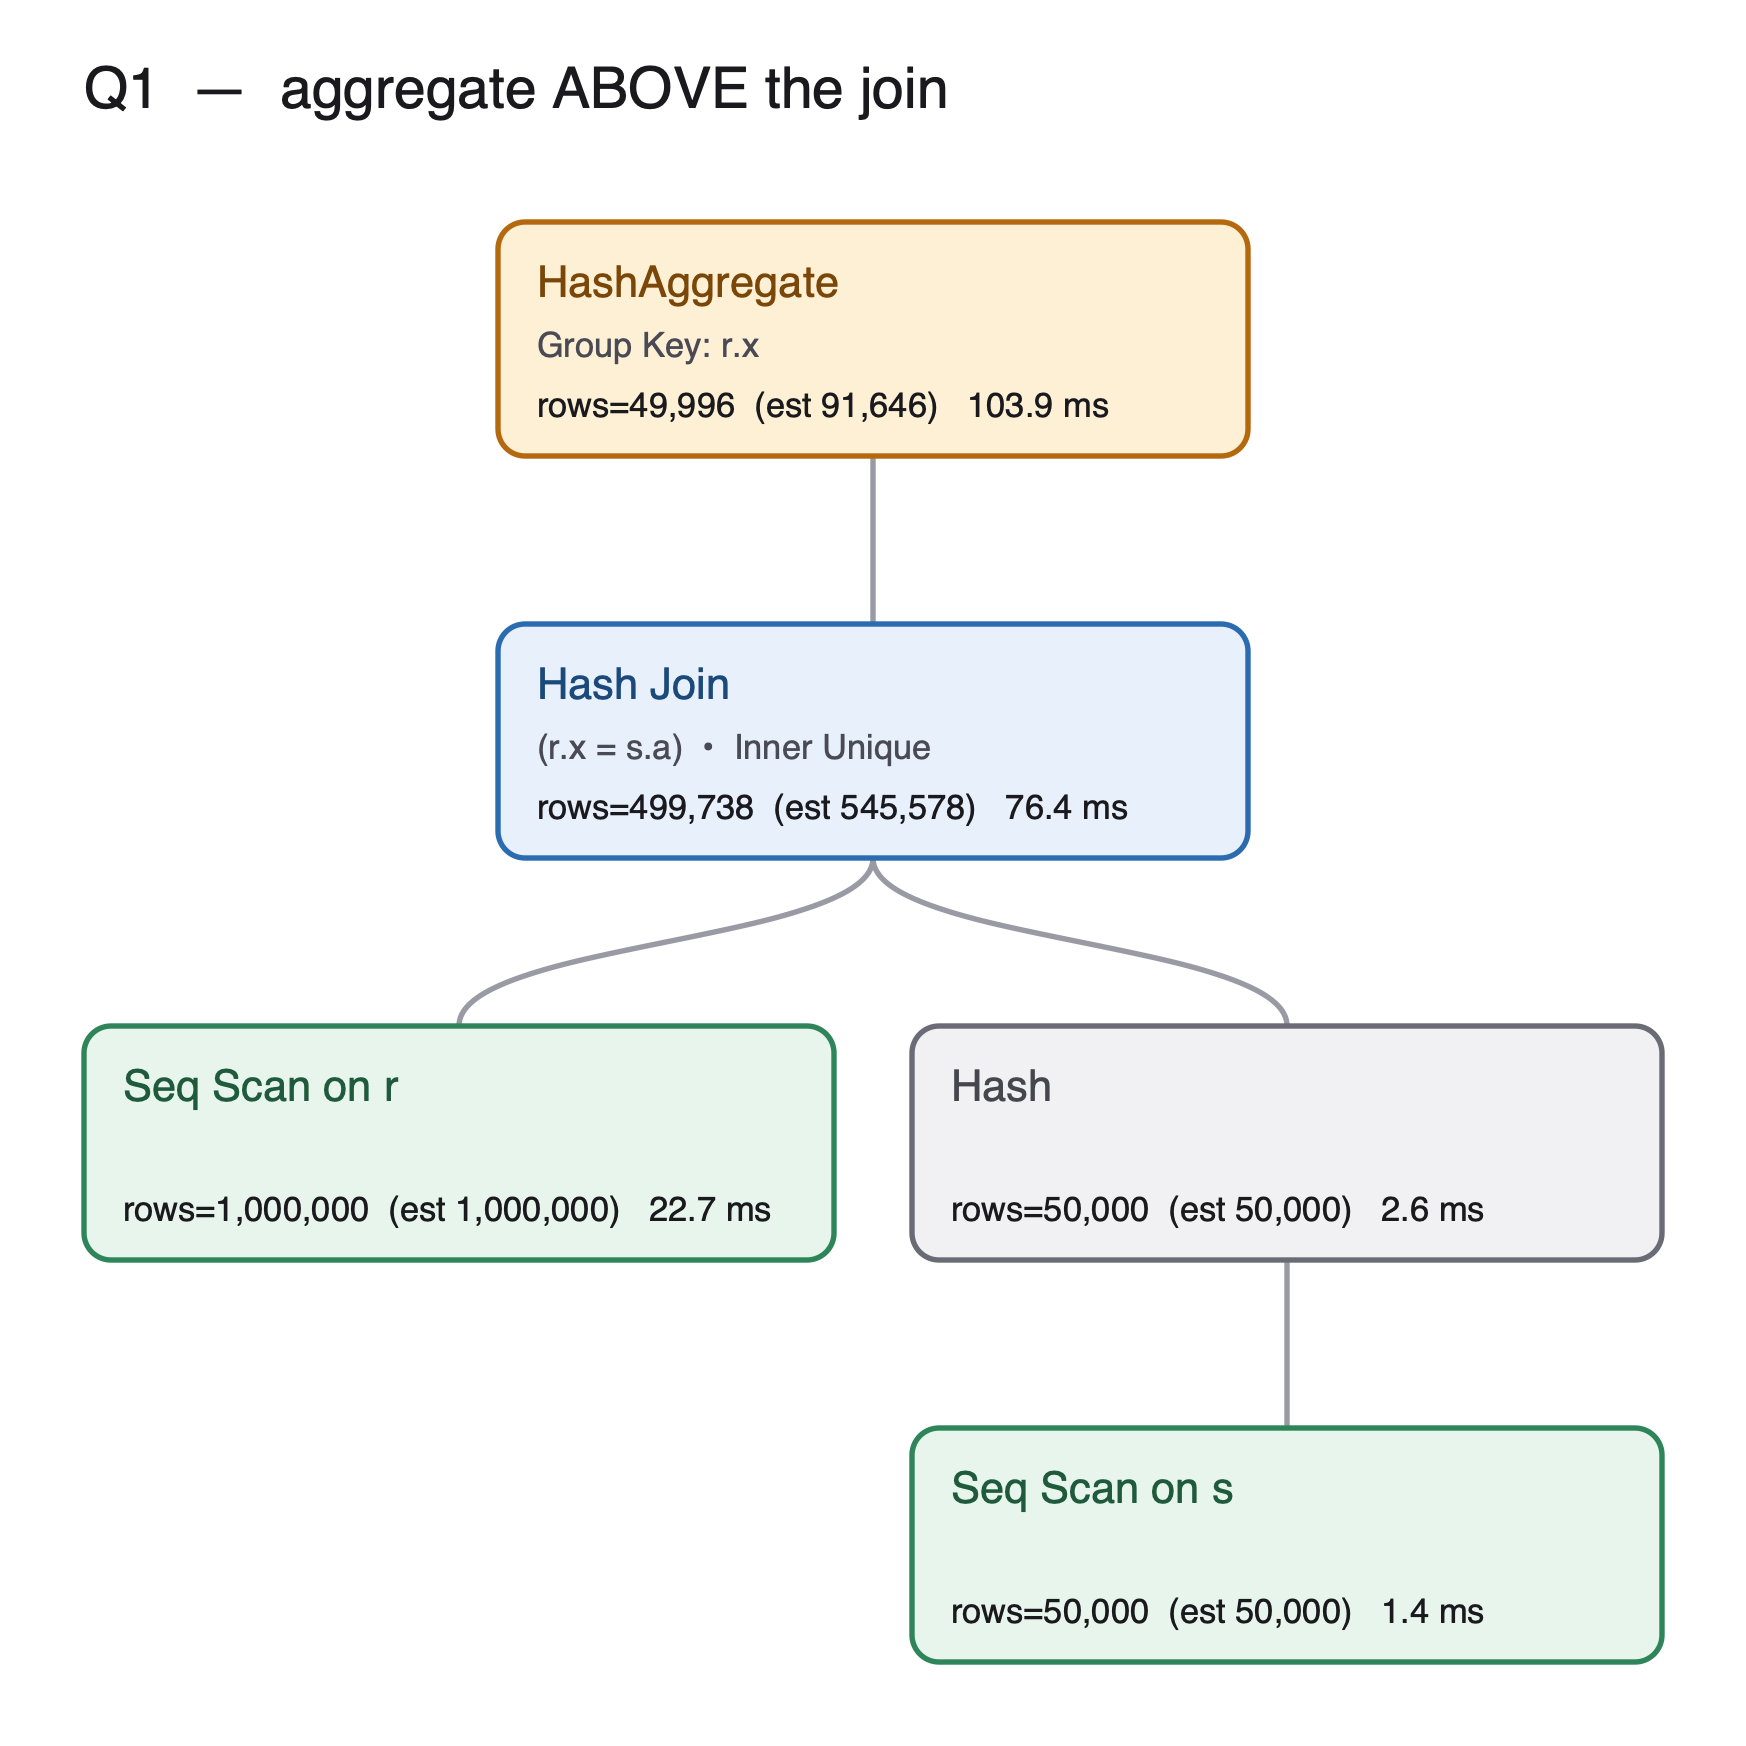
\includegraphics[width=0.47\linewidth]{figs/q1_plan.png}\hfill
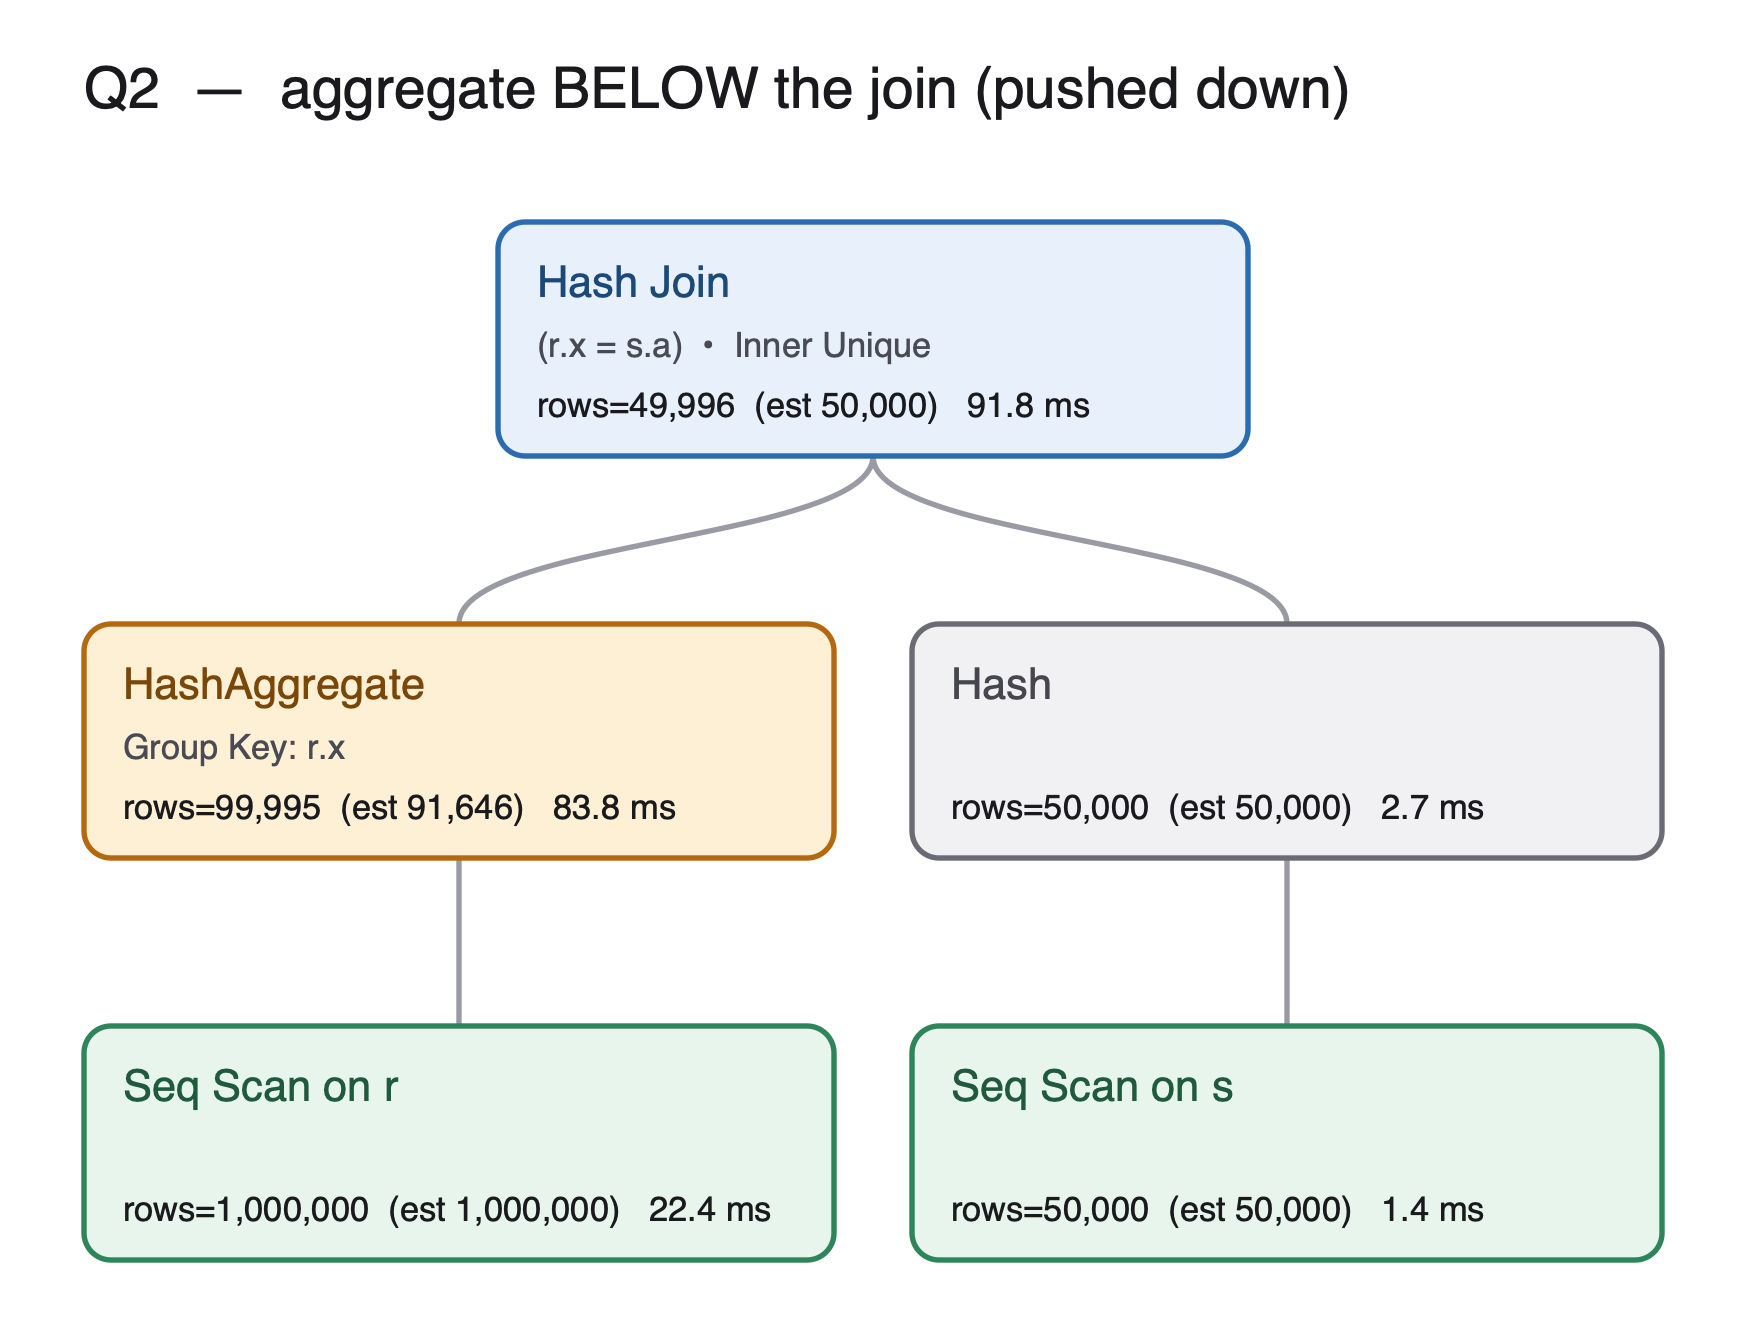
\includegraphics[width=0.47\linewidth]{figs/q2_plan.png}
\caption{PostgreSQL 18 \texttt{EXPLAIN (ANALYZE, VERBOSE, BUFFERS)} for $Q_1$ (left) and
$Q_2$ (right). Note \texttt{Inner Unique} on both joins: the planner read the primary key
and recorded ``at most one match on the inner side''. \emph{That flag is the same fact the
provers write as $\sq{S(a)}$} --- Postgres uses it to stop probing early, the provers use
it to justify the rewrite.}
\label{fig:pgplans}
\end{figure}

\begin{table}[h]\centering\small
\begin{tabular}{@{}lrr@{}}
\toprule
 & $Q_1$ (agg above) & $Q_2$ (agg below)\\
\midrule
rows entering the aggregate & 499{,}738 & 1{,}000{,}000\\
groups produced             & 49{,}996  & 99{,}995\\
rows entering the join      & 1{,}000{,}000 & 99{,}995\\
final rows                  & 49{,}996  & 49{,}996\\
execution time              & 105.5\,ms & 93.1\,ms\\
\bottomrule
\end{tabular}
\caption{Measured. The pushdown is only $\approx$12\% faster here and its aggregate does
\emph{more} work; the win comes from the join seeing 99{,}995 rows instead of $10^6$.
Whether to apply the rewrite is a cost question --- entirely separate from whether it is
\emph{correct}, which is what this document is about.}
\end{table}

\subsubsection{Why the primary key is load-bearing}
\label{sec:pkcounter}

Give $S$ a duplicate ($a=1$ twice, no key) and run the same two queries on the same $R$:

\begin{center}\small
\begin{tabular}{@{}lll@{}}
\toprule
 & result & rows\\\midrule
$Q_1$ (agg above join) & $(1,\,60)$ & 1\\
$Q_2$ (agg below join) & $(1,\,30),\ (1,\,30)$ & 2\\
\bottomrule
\end{tabular}
\end{center}

Not equivalent, and wrong in two independent ways:

\begin{itemize}
\item $Q_1$ joins first, so every $R$ row is duplicated \emph{before} the aggregate sees
      it. The bag entering \lstinline|SUM| becomes $\{10,10,20,20\}$ instead of
      $\{10,20\}$, so the \textbf{value} is corrupted: $60$ instead of $30$.
\item $Q_2$ aggregates first, so \lstinline|SUM| sees the clean bag. The duplication hits
      the \textbf{output row count} instead: two copies of $(1,30)$.
\end{itemize}

This is the same phenomenon Calcite compensated for in \S\ref{sec:calcite-fires}: with
$\mathrm{count} = 2$, Calcite's rewritten plan computes $30 \times 2 = 60$, matching $Q_1$.
On PostgreSQL, \texttt{Inner Unique} disappears from $Q_1$'s plan the moment the key is
dropped.

\keybox{The specification of the running example}{%
$Q_1 \equiv Q_2$ \textbf{if and only if} the join column on the right is distinct.
A prover that cannot turn ``\texttt{a} is a primary key'' into a usable algebraic fact
cannot prove this rewrite; one that proves it \emph{without} using the key is unsound.}

\section{U-expressions: the U-semiring and \udp{}}
\label{sec:uexpr}

\emph{Source: Chu, Murphy, Roesch, Cheung, Suciu, PVLDB 11(11), 2018~\cite{udp}.}

\subsection{The design goal, and the two constraints that shaped it}

The authors wanted an algebra in which SQL equivalence proofs are \emph{machine-checkable
down to axioms}, so they could be discharged in Coq. That imposes two constraints that
explain almost every design choice:

\begin{enumerate}
\item \textbf{Everything must be an identity} (an equation $E_1 = E_2$), not a logical
      sentence like $\forall t\,(\phi \Rightarrow \psi)$. Identities can be used as rewrite
      rules; implications need a theorem prover. This is why the key constraint gets the
      unusual definition in \S\ref{sec:key}.
\item \textbf{As few axioms as possible.} Fewer axioms means a smaller trusted base and a
      simpler proof search. The paper deliberately \emph{excludes} an order relation
      $\le$, even though $\le$ would make keys easy to state.
\end{enumerate}

\subsection{The U-semiring}

\begin{definition}[U-semiring, \cite{udp} Def.\ 3.1]
An \emph{unbounded semiring} is a structure
$(\Usemi,0,1,+,\times,\sq{\cdot},\notu{\cdot},(\usum{D})_{D\in\mathcal D})$ where
$(\Usemi,0,1,+,\times)$ is a commutative semiring and the extra operations satisfy the
axioms below.
\end{definition}

A commutative semiring is just ``arithmetic without subtraction'': $+$ and $\times$ are
associative and commutative, $0$ is the unit of $+$, $1$ the unit of $\times$, $\times$
distributes over $+$, and $0 \times x = 0$.

\paragraph{Squash $\sq{\cdot}$ (models \lstinline|DISTINCT|).}
\begin{align}
\sq{0} &= 0, &  \sq{1+x} &= 1 \label{ax:sq1}\\
\sq{\sq{x}+y} &= \sq{x+y} \label{ax:sq2}\\
\sq{x}\times\sq{y} &= \sq{x\times y} \label{ax:sq3}\\
\sq{x}\times\sq{x} &= \sq{x} \label{ax:sq4}\\
x \times \sq{x} &= x \label{ax:sq5}\\
x^2 = x &\;\Rightarrow\; \sq{x} = x \label{ax:sq6}
\end{align}

\paragraph{Negation $\notu{\cdot}$ (models \lstinline|NOT EXISTS|).}
\begin{align}
\notu{0} &= 1 \label{ax:not1}\\
\notu{x\times y} &= \sq{\notu{x}+\notu{y}} \label{ax:not2}\\
\notu{x+y} &= \notu{x}\times\notu{y} \label{ax:not3}\\
\notu{\sq{x}} &= \sq{\notu{x}} = \notu{x} \label{ax:not4}
\end{align}

\paragraph{Unbounded summation $\usum{t}$ (models projection).}
\begin{align}
\usum{t}\bigl(f_1(t)+f_2(t)\bigr) &= \usum{t}f_1(t) + \usum{t}f_2(t) \label{ax:s7}\\
\usum{t_1}\usum{t_2} f(t_1,t_2) &= \usum{t_2}\usum{t_1} f(t_1,t_2) \label{ax:s8}\\
x \times \usum{t} f(t) &= \usum{t} \bigl(x\times f(t)\bigr) \label{ax:s9}\\
\Bigl\lVert \usum{t} f(t) \Bigr\rVert &= \Bigl\lVert \usum{t} \sq{f(t)} \Bigr\rVert \label{ax:s10}
\end{align}

\paragraph{Predicates and equality.}
For each SQL predicate $b$ there is $\ind{b}\in\Usemi$ with
\begin{align}
\ind{b} &= \sq{\ind{b}} \label{ax:p11}
\intertext{and equality satisfies \emph{excluded middle}, \emph{substitution of equals} and
\emph{uniqueness}:}
\ind{e_1=e_2} + \ind{e_1\neq e_2} &= 1 \label{ax:p12}\\
f(e_1)\times\ind{e_1=e_2} &= f(e_2)\times\ind{e_1=e_2} \label{ax:p13}\\
\usum{t}\ind{t=e} &= 1 \label{ax:p14}
\end{align}

\begin{lemma}[the workhorse, \cite{udp} Eq.\ 15]\label{lem:15}
$\displaystyle \usum{t}\ind{t=e}\times f(t) = f(e).$
\end{lemma}
\begin{proof}
By \eqref{ax:p13}, $\usum{t}\ind{t=e}f(t) = \usum{t}\ind{t=e}f(e)$; by \eqref{ax:s9} pull
$f(e)$ out, giving $f(e)\times\usum{t}\ind{t=e}$; by \eqref{ax:p14} the sum is $1$.
\end{proof}

\keybox{Lemma \ref{lem:15} is the single most-used rule in the whole system}{%
It says: \emph{a summation whose body pins the summation variable to a value collapses to
that one value.} A join condition \lstinline|ON x = a| creates exactly such a pin, which is
why join conditions make summations disappear. \QED{} rediscovers this as ``stabilisation''
(\S\ref{sec:stabilise}) but finds the pin with an SMT solver instead of syntactically.}

\subsection{Which structures actually \emph{are} U-semirings?}

This matters for soundness. The paper gives four models~\cite[\S3.1]{udp}:
$\mathbb{N}$ (if all summation domains are finite);
$\Nbar = \mathbb{N}\cup\{\infty\}$ (for arbitrary domains, with $x+\infty=\infty$,
$0\times\infty=0$, $x\times\infty=\infty$ for $x\neq0$);
univalent types; and cardinal numbers.

$\Nbar$ is the one to keep in mind --- and note that \QED{} later takes $\Nbar$ as its
\emph{only} model rather than as one model among many. That single decision is most of the
difference between the two systems.

\begin{remark}[why no order relation]
One could define a key by ``every key value occurs at most once'', i.e.\
$\usum{t}R(t)\times\ind{t.k=e} \le 1$. But $\le$ requires an ordered semiring, adding
axioms. The paper instead finds an \emph{equational} formulation (\S\ref{sec:key}).
Beware: axioms that look obviously true may not be. The paper's counterexample is the
semiring of diagonal $2\times2$ matrices over $\Nbar$, in which the plausible rule
``if $x\neq0$ then $\sq{x}=1$'' fails.
\end{remark}

\subsection{Translating SQL into U-expressions}

Every query $q$ becomes a function $\den{q} : \Tup{\sigma}\to\Usemi$.

\begin{align*}
\den{R} &= \lam{t}{R(t)}\\
\den{\text{\texttt{SELECT * FROM R x, S y}}} &= \lam{(t_1,t_2)}{R(t_1)\times S(t_2)}\\
\den{\text{\texttt{SELECT * FROM R WHERE b}}} &= \lam{t}{\ind{b}\times R(t)}\\
\den{\text{\texttt{SELECT a FROM R}}} &= \lam{t}{\usum{t'}\ind{t'.a = t}\times R(t')}\\
\den{\text{\texttt{q1 UNION ALL q2}}} &= \lam{t}{\den{q_1}(t)+\den{q_2}(t)}\\
\den{\text{\texttt{DISTINCT q}}} &= \lam{t}{\sq{\den{q}(t)}}\\
\den{\text{\texttt{EXISTS q}}} &= \sq{\den{q}}, \qquad
\den{\text{\texttt{NOT EXISTS q}}} = \notu{\den{q}}
\end{align*}
Boolean connectives follow the same pattern: \texttt{AND} $\mapsto \times$,
\texttt{OR} $\mapsto +$, \texttt{NOT} $\mapsto \notu{\cdot}$.

\paragraph{Aggregates.}
\udp{} treats every aggregate as an \emph{uninterpreted function} applied to a
U-expression: $\mathrm{agg}(E)$ is a value expression usable inside a predicate, e.g.\
$\ind{\mathrm{agg}(E)=t.a}$. Nothing is known about it except congruence: equal arguments
give equal results. \lstinline|GROUP BY| is de-sugared into a correlated subquery
\cite[\S3.2]{udp}:

\begin{lstlisting}[style=sql]
SELECT x.k AS k, agg(x.a) AS a1 FROM R x GROUP BY x.k
-- becomes
SELECT y.k AS k,
       agg(SELECT x.a AS a FROM R x WHERE x.k = y.k) AS a1
FROM R y
\end{lstlisting}

\begin{remark}[an implementation trap]\label{rem:groupby}
As printed above (and in the paper), the outer query iterates over \emph{every} row of
\texttt{R}, so a key occurring twice yields two output rows --- but \lstinline|GROUP BY|
emits one row per \emph{distinct} key. A faithful de-sugaring needs
\lstinline|SELECT DISTINCT| on the outer query, i.e.\ a squash. \QED{} makes this explicit
in its \texttt{GroupBy} rule (\S\ref{sec:qsem}), where the group-non-empty factor is
wrapped in $\sq{\cdot}$. If you implement the de-sugaring literally you will get wrong
multiplicities.
\end{remark}

\subsection{Sum-Product Normal Form (SPNF)}

\begin{definition}[SPNF, \cite{udp} Def.\ 3.3]\label{def:spnf}
$E$ is in SPNF if $E = T_1+\cdots+T_n$ and each term has the shape
\[
T \;=\; \usum{t_1,\dots,t_m}\ \ind{b_1}\times\cdots\times\ind{b_k}
\;\times\; \sq{E_s} \;\times\; \notu{E_n} \;\times\; M_1\times\cdots\times M_j
\]
where each $M_i$ is a table application $R(t)$, each $\ind{b_i}$ a predicate,
\textbf{exactly one} squash factor $\sq{E_s}$ (omitted when $E_s=1$),
\textbf{exactly one} negation factor $\notu{E_n}$ (omitted when $E_n=0$), and
$E_s,E_n$ are themselves in SPNF.
\end{definition}

Think of SPNF as ``disjunctive normal form for bags'': a sum of products, all summations
hoisted to the front, all predicates to the left, all squashes fused into one.

\begin{theorem}[\cite{udp} Thm.\ 3.4]
Every U-expression can be rewritten into SPNF using only U-semiring axioms.
\end{theorem}

The rewrite system, applied left-to-right until fixpoint:
\begin{align*}
E_1\times(E_2+E_3) &\rightsquigarrow E_1E_2+E_1E_3 &
(E_1+E_2)\times E_3 &\rightsquigarrow E_1E_3+E_2E_3\\
E_1\times(E_2\times E_3) &\rightsquigarrow (E_1\times E_2)\times E_3 &
\cdots M\ind{b}\cdots &\rightsquigarrow \cdots \ind{b} M\cdots\\
\usum{t}(f_1+f_2) &\rightsquigarrow \usum{t}f_1+\usum{t}f_2 &
E\times\usum{t}f(t) &\rightsquigarrow \usum{t}E\times f(t)\\
\Bigl(\usum{t}f(t)\Bigr)\times E &\rightsquigarrow \usum{t}f(t)\times E &
\sq{E_1}\times\sq{E_2} &\rightsquigarrow \sq{E_1\times E_2}\\
\notu{E_1}\times\notu{E_2} &\rightsquigarrow \notu{E_1+E_2} &&
\end{align*}
Each rule is an axiom used in one direction; each strictly makes progress, so the system
terminates. Note how \eqref{ax:sq3} and \eqref{ax:not3} are exactly what let you
\emph{merge} multiple squashes and negations into the single ones Definition~\ref{def:spnf}
demands.

\subsection{Integrity constraints as identities}
\label{sec:key}

This is \udp{}'s most original contribution and the part most worth stealing.

\begin{definition}[KEY, \cite{udp} Def.\ 4.1]\label{def:key}
$R.k$ is a key iff for all $t,t'$:
\[
\ind{t.k = t'.k}\times R(t)\times R(t') \;=\; \ind{t=t'}\times R(t).
\]
\end{definition}

Why this is the right definition, in two steps. Set $t=t'$: the left becomes
$R(t)\times R(t)$ and the right $R(t)$, so $R(t)^2 = R(t)$, which over $\mathbb{N}$ forces
$R(t)\in\{0,1\}$ --- \emph{no duplicate rows}. Now take $t\neq t'$ with $t.k=t'.k$: the
right side is $0$, so $R(t)\times R(t')=0$, i.e.\ at most one of them is present ---
\emph{no two rows share a key}. Together:

\begin{theorem}[\cite{udp} Thm.\ 4.2]
Over the U-semiring $\mathbb{N}$, Definition~\ref{def:key} holds iff $R.k$ is a key in the
ordinary sense.
\end{theorem}

\begin{definition}[FOREIGN KEY, \cite{udp} Def.\ 4.4]\label{def:fk}
$S.k'$ references $R.k$ iff
$\;S(t') = S(t')\times\usum{t}R(t)\times\ind{t.k=t'.k'}$.
\end{definition}
Read it as: ``if $t'$ is in $S$ then multiplying by the number of matching $R$ rows changes
nothing'', which over $\mathbb{N}$ forces that number to be exactly $1$ whenever
$S(t')\neq0$.

\begin{theorem}[key implies squash-stability, \cite{udp} Thm.\ 4.3]\label{thm:43}
If $R.k$ is a key then for any $E$, $e$, $b$:
\[
\usum{t}\ind{b}\times\sq{E}\times\ind{t.k=e}\times R(t)
=\Bigl\lVert \usum{t}\ind{b}\times\sq{E}\times\ind{t.k=e}\times R(t)\Bigr\rVert.
\]
\end{theorem}
\begin{proof}[Proof sketch]
By \eqref{ax:sq6} it suffices to show the left side squared equals itself. Multiply
Definition~\ref{def:key} through by $\ind{b}^2\sq{E}^2$ (using $\ind{b}^2=\ind{b}$ and
$\sq{E}^2=\sq{E}$), sum over $t$ and $t'$, apply \eqref{ax:s9} twice on the left and
Lemma~\ref{lem:15} on the right.
\end{proof}

\noindent\textbf{Why Theorem~\ref{thm:43} matters:} it is the formal statement of
``a lookup by key returns at most one row''. It is what turns a key into a squash, and it
is the ancestor of \QED{}'s much simpler rule $S \rightsquigarrow \lam{a}{\sq{S(a)}}$.

\paragraph{Views and indexes.} A view becomes an assertion $v(t)=q(t)$ and is inlined. An
index on $R.a$ is modelled, GMAP-style, as the view
\lstinline|SELECT x.a, x.k FROM R x| where $k$ is the key --- then inlined too. So indexes
need no new machinery.

\subsection{A complete worked proof: the index rewrite}
\label{sec:udp-worked}

This is \cite[Ex.\ 4.7]{udp}, and it is the best single illustration of axiom-chasing.
$R$ has key $k$; $I$ is an index on $R.a$.

\begin{lstlisting}[style=sql]
-- Q1 : plain scan
SELECT * FROM R WHERE R.a >= 12
-- Q2 : index lookup
SELECT t2.* FROM I t1, R t2 WHERE t1.k = t2.k AND t1.a >= 12
\end{lstlisting}

$\den{Q_1}(t) = R(t)\times\ind{t.a\ge 12}$. Inlining $I$ and normalising to SPNF:
\[
\den{Q_2}(t)=\usum{t_1,t_2,t_3}
\ind{t_2=t}\ind{t_1.k=t_2.k}\ind{t_1.a\ge12}\ind{t_3.k=t_1.k}\ind{t_3.a=t_1.a}R(t_3)R(t_2).
\]

\begin{enumerate}
\item $t_1$ ranges over tuples of $I$'s schema, namely $(k,a)$. The two equalities
      $\ind{t_3.k=t_1.k}$ and $\ind{t_3.a=t_1.a}$ therefore \emph{determine} $t_1$
      completely: $\ind{t_1 = (t_3.k,t_3.a)}$. Apply Lemma~\ref{lem:15} to delete
      $\usum{t_1}$ and substitute:
      \[
      \usum{t_2,t_3}\ind{t_2=t}\ind{t_3.k=t_2.k}\ind{t_3.a\ge12}R(t_3)R(t_2).
      \]
\item Apply the KEY identity (Def.~\ref{def:key}) to
      $\ind{t_3.k=t_2.k}R(t_3)R(t_2) = \ind{t_2=t_3}R(t_2)$:
      \[
      \usum{t_2,t_3}\ind{t_2=t}\ind{t_3.a\ge12}R(t_2)\ind{t_2=t_3}.
      \]
\item Lemma~\ref{lem:15} on $t_3$ (pinned to $t_2$), then on $t_2$ (pinned to $t$):
      \[
      \den{Q_2}(t) = \ind{t.a\ge12}\times R(t) = \den{Q_1}(t).\qquad\blacksquare
      \]
\end{enumerate}

\keybox{The proof strategy in one sentence}{%
Put both queries in SPNF, then repeatedly (i) delete summations whose variable is pinned,
and (ii) apply constraint identities, until the two expressions are \emph{syntactically
identical}.}

\subsection{The decision procedure}

\udp{} is three mutually recursive procedures. Read them together with
Definition~\ref{def:spnf}; each procedure handles one layer of that grammar.

\begin{center}
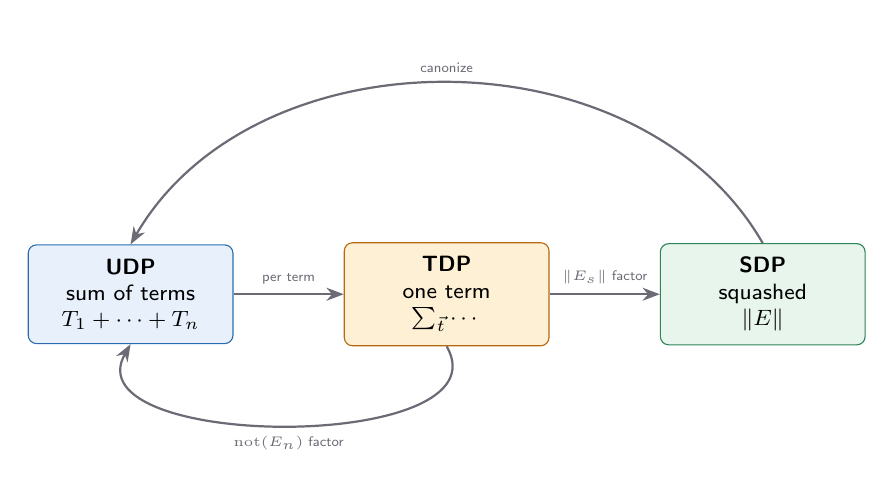
\begin{tikzpicture}[node distance=8mm,
  b/.style={draw=cGrey,fill=cGreyBg,rounded corners=3pt,inner sep=5pt,
            font=\footnotesize\sffamily,align=center,minimum width=26mm},
  ar/.style={-{Stealth[length=2.2mm]},cGrey,thick}]
\node[b,fill=cBlueBg,draw=cBlue] (u) {\textbf{UDP}\\sum of terms\\$T_1+\cdots+T_n$};
\node[b,fill=cAmberBg,draw=cAmber,right=14mm of u] (t) {\textbf{TDP}\\one term\\$\usum{\vec t}\cdots$};
\node[b,fill=cGreenBg,draw=cGreen,right=14mm of t] (s) {\textbf{SDP}\\squashed\\$\sq{E}$};
\draw[ar] (u)--node[above,font=\tiny\sffamily]{per term}(t);
\draw[ar] (t)--node[above,font=\tiny\sffamily]{$\sq{E_s}$ factor}(s);
\draw[ar] (t.south) to[out=-60,in=-120] node[below,font=\tiny\sffamily]{$\notu{E_n}$ factor} (u.south);
\draw[ar] (s.north) to[out=120,in=60] node[above,font=\tiny\sffamily]{canonize} (u.north);
\end{tikzpicture}
\end{center}

\paragraph{Step 0: canonize (\cite{udp} Alg.\ 1).}
Given $E$ in SPNF and constraint set $C$:
\begin{enumerate}
\item Close equality predicates under transitivity:
      $\ind{e_1{=}e_2}\ind{e_2{=}e_3} = \ind{e_1{=}e_2}\ind{e_2{=}e_3}\ind{e_1{=}e_3}$.
\item Repeatedly apply Lemma~\ref{lem:15} to delete pinned summations.
\item For each key constraint, rewrite with Def.~\ref{def:key} and Thm.~\ref{thm:43}.
\item For each foreign key, rewrite with Def.~\ref{def:fk}.
\end{enumerate}

\warnbox{Canonization may not terminate}{%
Steps 3--4 are a \emph{chase}. The paper says so explicitly: a cycle in the
key/foreign-key graph can loop forever. Their mitigation is pragmatic --- step 4 is applied
to squashed expressions only until the result stops changing (checked by calling
\textsc{SDP}), and elsewhere only until no new base relation is introduced. If you
implement this, put a depth bound on it.}

\paragraph{Step 1: \textsc{UDP} (\cite{udp} Alg.\ 2).}
\begin{lstlisting}[style=pseudo]
procedure UDP(E1, E2, C):
    E1 <- canonize(E1, C);  E2 <- canonize(E2, C)
    # E1 = T(1,1)+...+T(1,n),  E2 = T(2,1)+...+T(2,m)
    if m != n: return false                 # <-- the hard ceiling
    for each permutation p of E1's terms:
        if for all i: TDP(p[i], T(2,i), C): return true
    return false
\end{lstlisting}

\paragraph{Step 2: \textsc{TDP} (\cite{udp} Alg.\ 3).}
Two terms are compared by searching for a \emph{bijection} $h$ between their summation
variables; after substituting, the terms must match componentwise:
\begin{itemize}
\item \textbf{predicates:} $\ind{b_{1,1}}\cdots\ind{b_{1,k}} = \ind{b_{2,1}}\cdots\ind{b_{2,m}}$,
      decided by \emph{congruence closure} --- compute equivalence classes of variables and
      function applications and compare. E.g.\ $\ind{a{=}b}\ind{c{=}d}\ind{b{=}e}\ind{f(a){=}g(d)}$
      matches $\ind{a{=}b}\ind{a{=}e}\ind{c{=}d}\ind{f(e){=}g(c)}$ via the classes
      $\{a,b,e\},\{c,d\},\{f(a),f(e)\},\{g(c),g(d)\}$. Aggregates appearing in predicates are
      treated as uninterpreted functions here.
\item \textbf{squash factors:} $\sq{E_{1,1}}$ vs $\sq{E_{2,1}}$ by \textsc{SDP};
\item \textbf{negation factors:} by calling \textsc{UDP} recursively;
\item \textbf{table factors:} same number, and $M_{1,1},\dots,M_{1,j}$ \emph{identical} to
      $M_{2,1},\dots,M_{2,\ell}$.
\end{itemize}

\warnbox{Where \udp{} is weakest}{%
The predicate check is congruence closure over \emph{uninterpreted} functions. It proves
$\ind{a{=}b}\Rightarrow\ind{f(a){=}f(b)}$ but it does \emph{not} know arithmetic. So
$\ind{a+b=0}$ and $\ind{a=-b}$ are different predicates to \udp{}, and it fails. This one
limitation motivates both successors: \spes{} and \QED{} call an SMT solver here instead.}

\paragraph{Step 3: \textsc{SDP} (\cite{udp} Alg.\ 4).}
Under a squash, multiplicities do not matter, so \emph{set} reasoning applies. \textsc{SDP}
first flattens nested squashes using
\begin{lemma}[\cite{udp} Lem.\ 5.1]
$\sq{a\times\sq{x}+y} = \sq{a\times x+y}$ in any U-semiring.
\end{lemma}
then canonizes both sides and checks mutual containment --- but without an order relation
it cannot express containment directly. Instead it \emph{minimises} each term using only
U-semiring axioms (the analogue of conjunctive-query minimisation) and compares the minimal
forms syntactically:
\[
\forall i\,\exists j.\ \mathrm{minimize}(\sq{T_i})=\mathrm{minimize}(\sq{T'_j})
\ \wedge\
\forall j\,\exists i.\ \mathrm{minimize}(\sq{T'_j})=\mathrm{minimize}(\sq{T_i}).
\]

\begin{example}[\cite{udp} Ex.\ 5.2 --- self-join under DISTINCT]
\lstinline|SELECT DISTINCT x.a FROM R x, R y| $\;\equiv\;$ \lstinline|SELECT DISTINCT R.a FROM R|.
\[
Q_1(t)=\Bigl\lVert\usum{t_1,t_2}\ind{t_1.a=t}R(t_1)R(t_2)\Bigr\rVert
\]
Insert $1 = \ind{t_1{=}t_2}+\ind{t_1{\neq}t_2}$ by \eqref{ax:p12} and distribute:
\[
Q_1(t)=\Bigl\lVert\usum{t_1}\ind{t_1.a{=}t}R(t_1)R(t_1)
+\usum{t_1,t_2}\ind{t_1{\neq}t_2}\ind{t_1.a{=}t}R(t_1)R(t_2)\Bigr\rVert
\]
(the first sum used Lemma~\ref{lem:15} on $t_2$). By \eqref{ax:s10} and \eqref{ax:sq4},
$R(t_1)R(t_1)$ under a squash becomes $R(t_1)$. Factor with \eqref{ax:s7}/\eqref{ax:s9}:
\[
Q_1(t)=\Bigl\lVert\usum{t_1}\ind{t_1.a{=}t}R(t_1)\times\bigl(1+\usum{t_2}\ind{t_1{\neq}t_2}R(t_2)\bigr)\Bigr\rVert
\]
and by \eqref{ax:sq1} ($\sq{1+x}=1$) together with \eqref{ax:sq3}, the parenthesised factor
collapses, giving $\sq{\usum{t_1}\ind{t_1.a=t}R(t_1)} = Q_2(t)$.
\end{example}

\subsection{Guarantees}

\begin{theorem}[soundness, \cite{udp} Thm.\ 5.3]
If \textsc{UDP} returns true, the queries are equivalent under standard SQL semantics.
\end{theorem}
The argument is short because every step is an axiom application, and $\mathbb{N}$ is a
model of the axioms.

\begin{theorem}[completeness for UCQ]
\textsc{UDP} is complete when both inputs are unions of conjunctive queries, evaluated
under set semantics only, or under bag semantics only.
\end{theorem}
For a bag CQ \lstinline|SELECT p FROM R1 t1,...,Rn tn WHERE b| with $b$ a conjunction of
equalities, canonization yields the \emph{unique} canonical form
$\usum{t_1\ldots t_n}\ind{b}R_1(t_1)\cdots R_n(t_n)$; for the set version the same inside a
squash. Uniqueness plus the term-matching search gives completeness.

\begin{remark}[a genuine incompleteness, and it is interesting]
U-equivalence is \emph{stronger} than SQL equivalence, because U-semirings include models
with infinite relations. Take a first-order \emph{infinity axiom} $\varphi$ --- a sentence
false on every finite $R$ but satisfiable on an infinite one (e.g.\ ``$R$ is a non-empty,
injective, non-surjective function''). Encode $\varphi$ as a query $Q$ returning one row
when $\varphi$ holds and none otherwise. On every finite database $Q$ is equivalent to the
empty query, but they are \emph{not} U-equivalent, because they differ in the model $\Nbar$
with infinite support. So \udp{} must answer UNKNOWN. This is the price of keeping
unbounded summation primitive.
\end{remark}

\subsection{\udp{} on the running example --- and why it fails}
\label{sec:udp-fails}

Take $Q_1,Q_2$ from \S\ref{sec:running}. Two things go wrong, and both are structural.

\paragraph{(a) The aggregate is a black box compared out of context.}
After de-sugaring, both queries contain $\mathrm{Sum}$ applied to a U-expression. \udp{}
can conclude $\mathrm{Sum}(E_1)=\mathrm{Sum}(E_2)$ only by congruence, i.e.\ only if
$E_1$ and $E_2$ are equal \emph{as U-expressions}. Here
\[
E_1 = \lam{y}{R(x,y)\times\sq{S(x)}} \qquad\text{versus}\qquad E_2=\lam{y}{R(x,y)},
\]
and these are genuinely \emph{not} equal: when $x$ does not occur in $S$, the left is $0$
and the right is not. The recursive check is performed with no knowledge of the enclosing
context, so it fails --- correctly, but uselessly. Fixing this is precisely \QED{}'s
$\phi_1\vee\phi_2$ trick (\S\ref{sec:ambient}).

\paragraph{(b) Predicate matching is syntactic.}
Even the easy part --- deleting $\usum{a}$ using $\ind{x=a}$ --- only works when the pin is
syntactically visible. Write the join condition as \lstinline|x - a = 0| and \udp{} no
longer sees it.

\paragraph{What \udp{} \emph{can} do here.}
It handles the primary key fine: Theorem~\ref{thm:43} converts the key lookup into a
squash, exactly as needed. The key machinery is not the weak point --- the aggregate and
the syntactic predicate check are.

\subsection{Scorecard for U-expressions as of 2018}

\begin{table}[h]\centering\small
\begin{tabularx}{\linewidth}{@{}lX@{}}
\toprule
\textbf{Strong} & minimal axiom set, machine-checkable proofs, first equational treatment of
keys/foreign keys, UCQ-complete under set \emph{or} bag semantics, handles mixed
set/bag queries and \lstinline|NOT EXISTS|.\\
\midrule
\textbf{Weak} & syntactic predicate matching (no arithmetic); aggregates uninterpreted and
compared out of context; \lstinline|UDP| bails when the two sides have different numbers of
terms; canonization may not terminate; no NULL semantics at all, hence no outer joins;
proved 33--34 of the 232 Calcite pairs.\\
\bottomrule
\end{tabularx}
\end{table}

Both successors attack exactly one of these lists. \QED{} attacks ``no NULLs, no SMT,
context-free subquery checks''. \sqlsolver{} attacks ``different numbers of terms,
uninterpreted aggregates''.

\section{Q-expressions and \QED{}}
\label{sec:qexpr}

\emph{Source: Wang, Pan, Cheung, PVLDB 17(11):3602--3614, 2024~\cite{qed}.}

\subsection{The one-line summary}

Q-expressions have \emph{the same syntax} as U-expressions. What changes is that they are
pinned to a single concrete semantic domain, which makes every operator \emph{definable}
rather than axiomatised, which in turn makes them cheaply encodable into SMT. Everything
else in \QED{} follows from that.

\begin{table}[h]\centering\small
\begin{tabularx}{\linewidth}{@{}lXX@{}}
\toprule
 & \textbf{U-expression} & \textbf{Q-expression}\\
\midrule
semantics & any U-semiring; operators fixed by \emph{axioms} & the single model $\Nbar$; operators fixed by \emph{definitions}\\
$\sq{a}$ & 6 axiom lines (7 identities) & \emph{defined} as $\ind{a\neq0}$\\
$\notu{a}$ & 4 axiom lines & \emph{defined} as $\ind{a=0}$\\
decision & syntactic isomorphism & SMT, used at every stage\\
NULL & absent & first class (option types, 3-valued logic)\\
unknown operators & unsupported & $\qop$/$\hop$, first class\\
\bottomrule
\end{tabularx}
\end{table}

\subsection{The concrete domain}

\begin{definition}[\cite{qed} Eq.\ 4]\label{def:nbar}
Multiplicities live in $\Nbar=\mathbb{N}\cup\{\infty\}$ with
\[
\infty+a=\infty,\qquad 0\times\infty=0,\qquad a\times\infty=\infty\ (a\neq0),
\]
\[
\usum{s} f(s)=\begin{cases} f(s_1)+\cdots+f(s_n) & \text{if } \mathrm{supp}(f)=\{s_1,\dots,s_n\}\text{ is finite}\\ \infty & \text{otherwise,}\end{cases}
\]
\[
\ind{P}=\begin{cases}1&P\text{ true}\\0&\text{else,}\end{cases}
\qquad \sq{a}=\ind{a\neq0},\qquad \notu{a}=\ind{a=0}.
\]
A \emph{Q-expression} is any expression of type $\Nbar$.
\end{definition}

\keybox{Why this is more than bookkeeping}{%
$\Nbar$ \emph{is} a U-semiring, so nothing is lost. But because $\sq{a}$ is now literally
$\ind{a\neq0}$, a squash of a table application is just a Boolean --- an uninterpreted
predicate an SMT solver can reason about directly. In the axiomatic setting $\sq{\cdot}$ is
an opaque symbol you may only rewrite with the six squash axioms. This is the difference
between ``call Z3'' and ``search for an axiom chain''.}

\subsection{Query syntax}

\QED{} fixes a small relational core~\cite[Fig.\ 2]{qed}:
\[
\begin{array}{r@{\;}l@{\qquad}r@{\;}l}
Q ::=& \texttt{Table}(R:\sigma) & \mid& \texttt{Values}(v_1,\dots,v_n)\\
\mid& \texttt{Filter}(P,Q) & \mid& \texttt{Proj}(f,Q)\\
\mid& \texttt{Join}(Q_1,Q_2) & \mid& \texttt{Union}(Q_1,Q_2)\\
\mid& \texttt{Minus}(Q_1,Q_2) & \mid& \texttt{Distinct}(Q)\\
\mid& \texttt{GroupBy}(k,\alpha(f),Q) & \mid& \qop(o,v_1,\dots,v_n,Q)\\[4pt]
v,P,f ::=& x \mid \texttt{Exists}(Q) & \mid& \texttt{Op}(o,\vec v) \mid \hop(o,\vec v,Q)
\end{array}
\]
Two entries deserve comment.

$\qop$ and $\hop$ are \textbf{uninterpreted operators} --- \emph{first-class} escape
hatches. \lstinline|LIMIT 10| is $\qop(\texttt{Limit},10,Q)$; \lstinline|a IN Q| is
$\hop(\texttt{In},a,Q)$. Anything \QED{} does not model becomes one of these and still
participates in reasoning through congruence, rather than aborting the proof.

\begin{remark}[what is deliberately missing]
Set \texttt{Minus} and set \texttt{Intersect} are modelled; \emph{bag} minus and
\emph{bag} intersect are not. The paper's footnote is explicit: those would need a
\emph{monus} (truncated subtraction) at the semiring level, which \QED{} declines to add.
Handle them as $\qop$.
\end{remark}

\subsection{Semantics}
\label{sec:qsem}

\begin{align*}
\den{\texttt{Table}(R{:}\sigma)} &= \lam{x}{R(x)}\\
\den{\texttt{Values}(v_1..v_n)} &= \lam{x}{\ind{x{=}v_1}+\cdots+\ind{x{=}v_n}}\\
\den{\texttt{Filter}(P,Q)} &= \lam{x}{\ind{\den{P}(x)=\textsf{True}}\times\den{Q}(x)}\\
\den{\texttt{Proj}(f,Q)} &= \lam{x}{\usum{s}\ind{x=\den{f}(s)}\times\den{Q}(s)}\\
\den{\texttt{Join}(Q_1,Q_2)} &= \lam{x_1,x_2}{\den{Q_1}(x_1)\times\den{Q_2}(x_2)}\\
\den{\texttt{Union}(Q_1,Q_2)} &= \lam{x}{\den{Q_1}(x)+\den{Q_2}(x)}\\
\den{\texttt{Distinct}(Q)} &= \lam{x}{\sq{\den{Q}(x)}}\\
\den{\texttt{Minus}(Q_1,Q_2)} &= \lam{x}{\sq{Q_1(x)\times\notu{Q_2(x)}}}\\
\den{\texttt{GroupBy}(k,\alpha(f),Q)} &= \lam{x,y}{
   \underbrace{\Bigl\lVert\usum{s}\ind{x=\den{k}(s)}\times\den{Q}(s)\Bigr\rVert}_{\text{the group is non-empty}}
   \times \underbrace{\Bigl[\,y=\hop\bigl(\alpha,\lam{y'}{\usum{s}\den{Q}(s)\times\ind{x=\den{k}(s)\wedge y'=\den{f}(s)}}\bigr)\Bigr]}_{\text{$y$ is the aggregate of the group's bag}}}
\end{align*}
and for scalars, $\den{\texttt{Exists}(Q)}=\sq{\usum{s}\den{Q}(s)}$.

\paragraph{Read the \texttt{GroupBy} rule slowly --- it is the crux of the paper.}
The output row is the pair $(x,y)$ = (group key, aggregate value). Two factors:
\begin{itemize}
\item The \emph{squashed} sum says ``at least one input row has key $x$'', and the squash is
      what makes \lstinline|GROUP BY| emit \textbf{one} row per key regardless of input
      multiplicities. (This is exactly the subtlety \udp{}'s de-sugaring glosses over ---
      Remark~\ref{rem:groupby}.)
\item The bracket pins $y$ to $\alpha$ applied to a \emph{bag}: the function
      $\lam{y'}{\dots}$ whose value at $y'$ is the multiplicity of $y'$ within the group.
      $\alpha$ is an $\hop$, i.e.\ \textbf{uninterpreted}. \QED{} knows only that equal bags
      give equal aggregates.
\end{itemize}

\begin{definition}[the equivalence problem]
Write $\Gamma\mid\Delta\mid\Phi \vdash Q_1 \stackrel{?}{=} Q_2$, where $\Gamma$ are table
symbols, $\Delta$ other uninterpreted symbols and $\Phi$ an assumed predicate. It asks
whether $\den{Q_1}(s)=\den{Q_2}(s)$ for all instantiations of $\Gamma,\Delta$ satisfying
$\Phi$ and all rows $s$.
\end{definition}

\subsection{Integrity constraints: rewrite the table, not the query}

\paragraph{Primary key (\cite{qed} Eqs.\ 6--8).}
Let $R$ have schema $K\times S$ with key column(s) $k$. A table with a primary key is
\emph{exactly} a subset of $K$ plus a function $f_R:K\to S$ giving the non-key columns.
Formally, for any predicate $P$ over tables,
\begin{equation}\label{eq:pk-complete}
\forall R \text{ with primary key } k.\ P(R)
\iff \forall R',f_R.\ P\bigl(\lam{k,s}{\sq{R'(k)}\times\ind{s=f_R(k)}}\bigr)
\end{equation}
which licenses the rewrite
\begin{equation}\label{eq:pk7}
R \;\rightsquigarrow\; \lam{k,s}{\sq{R'(k)}\times\ind{s=f_R(k)}}
\end{equation}
introducing a fresh table symbol $R'$ of schema $K$ and a fresh function symbol $f_R$.
When $k$ is the \emph{only} column this collapses to the form everyone quotes:
\begin{equation}\label{eq:pk8}
R \;\rightsquigarrow\; \lam{k}{\sq{R(k)}}.
\end{equation}

\warnbox{Do not quote Eq.~\eqref{eq:pk8} when the table has non-key columns}{%
In our running example $S$ has schema $(a,b)$ with key $a$, so the applicable rule is
\eqref{eq:pk7}: $S\rightsquigarrow\lam{a,b}{\sq{S'(a)}\times\ind{b=f_S(a)}}$.
The familiar $\lam{a}{\sq{S(a)}}$ appears only after $b$ is projected away --- which the
queries do, since neither mentions $S.b$. The distinction matters the moment a query reads
a non-key column.}

The word \emph{complete} in the paper is Eq.~\eqref{eq:pk-complete}: the rewrite yields an
equivalence problem that is equivalent to the original, not merely implied by it. Contrast
\spes{}, whose primary-key support is a finite list of query-level rewrite rules --- sound,
but only firing on shapes someone anticipated.

\paragraph{Foreign key (\cite{qed} Eq.\ 9).}
\[
S \;\rightsquigarrow\; S,R' \mid \forall b,k.\ \sq{S(b,k)}\to\sq{R'(k)} \;\vdash\; S
\]
Note what changed relative to \udp{}: \udp{} applies its foreign-key identity
\emph{eagerly} as a rewrite, which does not terminate when two tables reference each other.
\QED{} emits \emph{one global logical formula} instead and lets the SMT solver unfold its
consequences lazily. That is a strictly better engineering decision and removes \udp{}'s
non-termination hazard.

\paragraph{Check constraint.} $\forall s.\ \sq{R(s)}\to C(s)$. One line, same idea.

\subsection{NULL semantics}

\udp{} has none; this alone rules out outer joins. \QED{} lifts every type $T$ to
$\mathrm{Option}(T)$, an algebraic datatype modern SMT solvers support natively.

\begin{itemize}
\item \textbf{Strict by default:} an $n$-ary operation returns \textsf{Null} exactly when
      some argument is \textsf{Null}. This lifts $+$, $\times$, comparisons, etc.
\item \textbf{Three-valued \texttt{AND}/\texttt{OR}} are the documented exceptions:
\begin{align*}
a\ \texttt{And}\ b &\coloneqq \mathrm{ite}(a=\textsf{Null},\ \mathrm{ite}(b=\textsf{True},\textsf{Null},b),\ \mathrm{ite}(a=\textsf{True},b,a))\\
a\ \texttt{Or}\ b &\coloneqq \mathrm{ite}(a=\textsf{Null},\ \mathrm{ite}(b=\textsf{False},\textsf{Null},b),\ \mathrm{ite}(a=\textsf{False},b,a))
\end{align*}
      Check them: \textsf{Null} \texttt{And} \textsf{False} $=$ \textsf{False} (not
      \textsf{Null}), and \textsf{Null} \texttt{Or} \textsf{True} $=$ \textsf{True}.
      Strictness would get both wrong.
\item \textbf{Quantified comparison:}
\[
a\ \langle\mathrm{cmp}\rangle\ \texttt{Some}\ Q \coloneqq
\mathrm{ite}\bigl(\exists x.\sq{Q(x)}\wedge (x\,\langle\mathrm{cmp}\rangle\,a)=\textsf{True},\ \textsf{True},\
\mathrm{ite}(\exists x.\sq{Q(x)}\wedge(x\,\langle\mathrm{cmp}\rangle\,a)=\textsf{Null},\ \textsf{Null},\ \textsf{False})\bigr)
\]
      \lstinline|a IN Q| is the special case with $\langle\mathrm{cmp}\rangle$ being
      \texttt{=}. The nesting order encodes SQL's rule: \emph{a true match wins over a
      null one}, and only if there is no match at all and no null do you get
      \textsf{False}.
\item \textbf{\lstinline|COUNT(*)| vs \lstinline|COUNT(k)|:} modelled by optionally applying
      a non-\textsf{Null} filter before the aggregate.
\end{itemize}

\subsection{Algorithm A: the complete fragment}
\label{sec:qed-complete}

\QED{} has \emph{two} algorithms and picks between them. The first is complete on a
restricted fragment; this is the paper's theoretical contribution.

\begin{definition}[$\mathcal F_T$, \cite{qed} Def.\ 1]
Fix a first-order theory $T$. The fragment $\mathcal F_T$ consists of
\texttt{Table}, \texttt{Values}, \texttt{Filter}, \texttt{Proj}, \texttt{Join},
\texttt{Union}, where all values, projection functions and filter predicates are definable
in $T$. Primary keys on the tables are allowed.
\end{definition}

This generalises Cohen's classical UCQ result~\cite{cohen}: UCQ forces predicates to be
conjunctions of (in)equalities and projections to be bare column references, whereas
$\mathcal F_T$ allows \emph{anything expressible in $T$}. With $T$ = the SMT solver's
theories, that is a large class. Note $\mathcal F_T$ excludes \texttt{GroupBy},
\texttt{Distinct} and \texttt{Minus} --- so our running example is \emph{not} in it.

\subsubsection{Scoped normal form (SNF)}
\begin{definition}[\cite{qed} Def.\ 2]
$U$ is in SNF if $U=T_1+\cdots+T_n$ where each \emph{normal term} is
\[
T=\usum{R_1^{k_1}(s_1)}\cdots\usum{R_m^{k_m}(s_m)} \ind{P},
\qquad
\usum{R^0(s)}U \coloneqq \usum{s}\sq{R(s)}\times U,\quad
\usum{R^k(s)}U \coloneqq \usum{s}\underbrace{R(s)\cdots R(s)}_{k}\times U
\]
with $P$ (the \emph{body}, $\mathrm{Bdy}\,T$) containing no table variables, and the
summations ordered consistently with a fixed order on table symbols.
\end{definition}
Auxiliary notation used below: $\mathrm{Scp}\,T$ is the list of all summation variables;
$\mathrm{Scp}_R T$ those attached to table $R$; $\mathrm{Rel}\,T$ the list of table
variables with their powers; $\mathrm{Rel}'T$ the same without powers.

\noindent Normalisation (\cite{qed} Alg.\ 1) is a straightforward induction:
\texttt{Table} is already a term; \texttt{Filter} conjoins its predicate into every body;
\texttt{Proj} post-composes $f$ into the body \emph{without} adding a summation;
\texttt{Join} merges scopes and conjoins bodies pairwise; \texttt{Union} concatenates terms.

\subsubsection{Linearisation (LNF)}
Two obstacles remain. First, summation variables attached to the same table can be
introduced in any order, so terms that differ only by a permutation look different.
Second, redundant variables: in
\[
T_1=\usum{R(s_1)}\usum{R(s_2)}\ind{(x{=}s_2)\wedge(s_1{=}s_2)}
\qquad\text{vs}\qquad
T_2=\usum{R^2(s_1)}\ind{x{=}s_1}
\]
$T_1$'s $s_2$ is redundant, but the scopes have different lengths so they cannot be
compared directly.

\begin{definition}[LNF, \cite{qed} Def.\ 3]
$U$ is in LNF if it is in SNF and, for every term $T$ and table variable $R$, $\mathrm{Bdy}\,T$
implies the variables of $\mathrm{Scp}_R T$ are pairwise distinct and form a linearly
ordered chain.
\end{definition}

Algorithm 2 achieves this by \emph{case-splitting on the order}. For a scope
$\{a,b,c\}$, $\mathrm{Lin}$ enumerates all $13$ ways three values can be ordered-or-equal
($a{<}b{<}c$, \dots, $a{=}b{<}c$, \dots, $a{=}b{=}c$). Each term is replaced by the sum over
all cases; within each case, variables proved equal are merged (the oracle decides
$\mathrm{Bdy}\,T'\to s_j=s_k$), and the survivors are sorted ascending. Now every term has a
canonical variable order.

\begin{remark}[cost]
$|\mathrm{Lin}(X)|$ is the ordered Bell number of $|X|$: $1, 1, 3, 13, 75, 541,\dots$
Eager linearisation is therefore expensive, which is exactly why \QED{}'s \emph{general}
algorithm (\S\ref{sec:qed-general}) defers permutation to the matching step instead.
\end{remark}

\subsubsection{Unification and completeness}
Terms are grouped by relational scope; within a group the summation disappears and only the
bodies are compared, because
\[
\usum{S}\ind{P_1}+\cdots+\ind{P_n} \;=\; \usum{S}\ind{P'_1}+\cdots+\ind{P'_m}
\quad\Longleftarrow\quad
\vec s \vdash_{\mathcal O} \ind{P_1}+\cdots+\ind{P_n} = \ind{P'_1}+\cdots+\ind{P'_m}
\]
and the right-hand side is an ordinary SMT query ($\ind{\cdot}$ becomes \texttt{ite},
$+$ becomes integer addition).

\begin{theorem}[\cite{qed} \S4.4]
On $\mathcal F_T$, with a complete oracle for $T$,
$\den{Q_1}=\den{Q_2}\Rightarrow \textsf{unify}(\textsf{lin}(\textsf{snf}(Q_1)),\textsf{lin}(\textsf{snf}(Q_2)))$.
\end{theorem}
\begin{proof}[Proof idea --- worth understanding, it is elegant]
Contrapositive. Suppose some group of terms with relational scope $S^*$ fails its body
check; choose such $S^*$ with the fewest variables. Build a database instance in which each
table $R_i$ is supported on exactly the finitely many points that the failing assignment
$\sigma$ touches, with multiplicity $n_i$ a free parameter. Because the term is in LNF, all
variables attached to a table are distinct and ordered, so a group with scope
$R_1^{k_1}\cdots R_m^{k_m}$ evaluates to the \emph{monomial}
$B_S[\delta,\sigma]\times n_1^{k_1}\cdots n_m^{k_m}$. Terms with larger scopes vanish (some
variable is forced outside the support). Both sides are thus polynomials in
$n_1,\dots,n_m$, and two polynomials over $\mathbb{N}$ are equal iff all coefficients match
--- but the $S^*$ coefficient differs by assumption. Hence some instantiation separates
$Q_1$ and $Q_2$.
\end{proof}

\keybox{The idea to steal}{%
LNF turns each term into a monomial whose exponents are the scope and whose coefficient is
the body. Bag equivalence then becomes \emph{polynomial identity}. That is why the paper
insists on a total order on summation variables: without it the exponents are not
well-defined.}

\subsection{Algorithm B: the general algorithm}
\label{sec:qed-general}

For everything outside $\mathcal F_T$ --- including our running example, which has
\texttt{GroupBy} --- \QED{} uses a weaker but far more general pipeline:
\textbf{normalise $\to$ stabilise $\to$ unify}. Here the oracle is allowed to answer
``unknown''.

\subsubsection{SPNF (\cite{qed} Alg.\ 4)}
Terms take the shape $\usum{\vec s}\ind{L}\times V$. The conversion is structural, and the
two interesting lines are
\[
\textsf{spnf}(\sq{V}) = \ind{\textsf{spnf}(V)\neq 0},
\qquad
\textsf{spnf}(\notu{V}) = \ind{\textsf{spnf}(V)=0},
\]
i.e.\ squash and negation are \emph{eliminated} in favour of predicates. Products merge
scopes and conjoin the conditions; sums concatenate.

\subsubsection{Stabilisation (\cite{qed} Alg.\ 5)}
\label{sec:stabilise}
This is \QED{}'s replacement for \udp{}'s Lemma~\ref{lem:15}, and the upgrade is that it is
\emph{semantic}. For each term $\usum{\vec s}\ind{L}\times V$ and each variable $s_i$, ask
whether $L$ implies $s_i = f(\text{other variables})$ for some expression $f$; if so,
substitute and delete the summation.

\begin{lstlisting}[style=pseudo]
function stable(U):
  U' <- 0
  for each term (Sum over s) [L] x V of U:
    s',L',V' <- s,L,V
    for each variable s_i in s:
      s'' <- s' minus s_i
      if exists f with  Gamma|Delta,s' |Phi |-_O  L' -> f(s'') = s_i :
         s' <- s'' ;  L' <- L'[f(s'')/s_i] ;  V' <- V'[f(s'')/s_i]
    U' <- U' + (Sum over s') [L'] x V'
  return U'
\end{lstlisting}

Two ways to find $f$ are given: synthesise it with SyGuS, or ask the SMT solver for the
\emph{congruence classes} of the term's subexpressions and read off an equal expression.
\QED{} implements the second for simplicity and reports the two are equally powerful in
practice.

\begin{example}[composing two projections]
$\usum{y,z}\ind{x=f(y)\wedge y=g(z)}R(z) \stackrel{?}{=} \usum{z}\ind{x=f(g(z))}R(z)$.
Congruence classes on the left over $\{x,y,z,f(y),g(z)\}$ are $\{x,f(y)\},\{y,g(z)\},\{z\}$,
exposing $y=g(z)$, so $y$ is eliminated. On the right the classes are $\{x,f(g(z))\},\{z\}$
and nothing is eliminated. The scopes now match.
\end{example}

\begin{remark}[a real, acknowledged gap]
The congruence-class method finds only expressions \emph{already present} in the term.
Given $\ind{x+3=10}$ it will not discover $x=7$, because $7$ never appears; SyGuS would.
The paper reports this never mattered in the evaluation.
\end{remark}

\subsubsection{Unification (\cite{qed} Alg.\ 6)}
\begin{lstlisting}[style=pseudo]
function unify(U1, U2):
  drop terms whose body is provably false (oracle: not (L and squash V))
  if #terms(U1) != #terms(U2): return Unknown       # <-- ceiling of THIS algorithm
  for each term T1 of U1:
     find a term T2 of U2 with termEq(T1,T2); remove it; else return Unknown
  return True

function termEq( (Sum s1)[L1] x V1 , (Sum s2)[L2] x V2 ):
  if len(s1) != len(s2): return False
  for each bijection sigma from s2 to s1:            # capped at 24 in the implementation
     L2,V2 <- L2[sigma], V2[sigma]
     L1',V1',L2',V2' <- ... with every HOp/QOp replaced by a FRESH variable
     C <- congruence facts obtained by recursively unifying those operators' arguments
          under the extra assumption  Phi and (L1' or L2')
     if  Phi and C  |-_O  [L1'] x V1' = [L2'] x V2' : return True
  return False
\end{lstlisting}

Three mechanisms are packed in here; take them one at a time.

\paragraph{(i) Scope permutation.} Summation is commutative, so before comparing bodies you
must try bijections between the two scopes. The justification is
$(\forall \vec s.\ f(\vec s)=g(\vec s)) \Rightarrow \usum{\vec s}f=\usum{\vec s}g$. Note
this is \emph{pointwise} comparison: sound, but it can only ever prove sums equal by proving
their summands equal. The implementation caps at 24 permutations; empirically only $\sim$2\%
of cases need more than the identity permutation.

\paragraph{(ii) Higher-order operators become fresh variables.}
$\qop(o,\vec v,\lam{x}{W})$ becomes a fresh table symbol; $\hop(o,\vec v,Q)$ a fresh scalar.
Congruence facts like $\forall x.R(x)=R'(x)$ are then \emph{recovered} by checking that the
operators match and recursively comparing their arguments.

\paragraph{(iii) The ambient assumption --- the genuinely new idea.}
\label{sec:ambient}
The recursive comparison of the operators' arguments is performed under the extra hypothesis
$L'_1\vee L'_2$: the conditions of the two enclosing terms. Soundness in one sentence:

\begin{lemma}[\cite{qed} Eq.\ 17]
To verify $\ind{L'_1}\times V'_1=\ind{L'_2}\times V'_2$ it suffices to check
$\Phi\wedge(L'_1\vee L'_2)\vdash C$ and $\Phi\wedge C\vdash \ind{L'_1}V'_1=\ind{L'_2}V'_2$.
\end{lemma}
\begin{proof}
If $\neg L'_1\wedge\neg L'_2$ then $\ind{L'_1}=\ind{L'_2}=0$ and both sides are $0$
regardless of $C$. So assuming $L'_1\vee L'_2$ while deriving $C$ loses nothing.
\end{proof}

\subsubsection{Encoding to first-order logic}
$\Nbar$-valued expressions cannot be handed to an SMT solver directly, but \QED{} never
needs their values --- only whether they are zero. So $U\neq0$ is pushed inward:
\[
U_1+U_2\neq0 \rightsquigarrow U_1\neq0\vee U_2\neq0,\qquad
U_1\times U_2\neq0 \rightsquigarrow U_1\neq0\wedge U_2\neq0,
\]
\[
\sq{U}\neq0\rightsquigarrow U\neq0,\qquad
\ind{P}\neq0\rightsquigarrow P,\qquad
\usum{s}U\neq0\rightsquigarrow \exists s.\,U\neq0.
\]
What survives is only fully-applied table symbols $R(a)\neq0$ and operator applications, all
of which are uninterpreted predicates. \QED{} additionally assumes every table has
\emph{finite} multiplicity at each row (type $S\to\mathbb{N}$, not $S\to\Nbar$) so that no
$\infty$ arises during term comparison.

\warnbox{This trick only works under a squash}{%
Turning $\usum{}$ into $\exists$ requires that the enclosing context care about
zero-vs-non-zero. When the top-level expression is \emph{not} squashed --- plain
\lstinline|SELECT x FROM r|, an unsquashed join --- multiplicities matter and \QED{} must
fall back on pointwise term matching, which is where its incompleteness bites
(\S\ref{sec:compare}).}

\begin{remark}[the two algorithms differ exactly here --- do not conflate them]
Alg.~6 demands a \emph{bijection} between the two sides' terms. Alg.~3, the
complete-fragment algorithm of \S\ref{sec:qed-complete}, does \textbf{not}: it groups terms
by relational scope and compares $\ind{P_1}+\cdots+\ind{P_n}$ with
$\ind{P'_1}+\cdots+\ind{P'_m}$ for $n\neq m$. So ``\QED{} cannot handle differing numbers of
terms'' is a statement about Alg.~6 only. A \lstinline|UNION ALL| split stays provable while
the query remains inside $\mathcal F_T$; adding a \texttt{GroupBy} or \texttt{Distinct}
pushes it into Alg.~6 and the bijection requirement returns.
\end{remark}

\subsection{The running example, proved}
\label{sec:qed-worked}

Translate $Q_1,Q_2$ of \S\ref{sec:running}, with the primary key already applied:
\begin{align*}
Q_1(x,r) &= \Bigl\lVert\usum{y,a}\ind{x{=}a}R(x,y)\sq{S(a)}\Bigr\rVert
 \times\Bigl[r=\Sumagg\bigl(\lam{y}{\usum{a}\ind{x{=}a}R(x,y)\sq{S(a)}}\bigr)\Bigr]\\
Q_2(x,r) &= \usum{a}\ind{x{=}a}\ \Bigl\lVert\usum{y}R(x,y)\Bigr\rVert
 \times\bigl[r=\Sumagg(\lam{y}{R(x,y)})\bigr]\times\sq{S(a)}
\end{align*}

\paragraph{Step 1 --- stabilise.} Both terms contain $\ind{x=a}$, which pins $a$ to $x$;
congruence classes put $x$ and $a$ together, so $\usum{a}$ is deleted:
\begin{align*}
Q_1(x,r) &= \Bigl\lVert\usum{y}R(x,y)\sq{S(x)}\bigl[r=\Sumagg(\lam{y}{R(x,y)\sq{S(x)}})\bigr]\Bigr\rVert\\
Q_2(x,r) &= \Bigl\lVert\usum{y}R(x,y)\sq{S(x)}\bigl[r=\Sumagg(\lam{y}{R(x,y)})\bigr]\Bigr\rVert
\end{align*}
One difference remains: the $\sq{S(x)}$ inside the aggregate.

\begin{remark}[why $Q_2$ may be written with an outer squash]
Every factor of $Q_2$ is already $0$-or-$1$: $\sq{\usum{y}R(x,y)}$, the bracket, and
$\sq{S(a)}$. So wrapping in $\sq{\cdot}$ changes nothing. But $\sq{S(a)}$ is squashed
\emph{only because of the primary key} --- drop the key and the factor is $S(a)$, which can
be $2$, and $Q_2$ is no longer squashable. That is precisely the counterexample of
\S\ref{sec:pkcounter}, where $Q_2$ returned $(1,30)$ \emph{twice}.
\end{remark}

\paragraph{Step 2 --- encode.} With $v_1,v_2$ fresh for the two aggregates:
\[
\phi_1(x,r)=\exists y.\,R(x,y)\neq0\wedge S(x)\neq0\wedge r=v_1,\qquad
\phi_2(x,r)=\exists y.\,R(x,y)\neq0\wedge S(x)\neq0\wedge r=v_2
\]
Goal $\forall x,r.\ \phi_1\leftrightarrow\phi_2$; identical but for $v_1$ vs $v_2$.

\paragraph{Step 3 --- recursive check with the ambient assumption.}
$v_1=v_2$ needs $\lam{y}{R(x,y)\sq{S(x)}}\equiv\lam{y}{R(x,y)}$, which is \textbf{false}
standalone ($x\notin S \Rightarrow$ left is empty). Under $\phi_1\vee\phi_2$, however, we
have $S(x)\neq0$, hence $\sq{S(x)}=1$, hence
\[
(\phi_1\vee\phi_2)\rightarrow\forall y.\ R(x,y)\times\sq{S(x)}=R(x,y)
\qquad\text{\emph{valid}.}
\]
So $v_1=v_2$, so $\phi_1\leftrightarrow\phi_2$, so $Q_1\equiv Q_2$. $\blacksquare$

\medskip
\noindent In English: \emph{the group-by only emits a row for an $x$ that survived the join,
and any such $x$ is in $S$; so inside the aggregate $\sq{S(x)}$ is just $1$ and vanishes.}

\subsection{Results and honest limits}

\begin{table}[h]\centering\small
\begin{tabular}{@{}llrrrrr@{}}
\toprule
suite & & \udp{} & EQUITAS & \spes{} & $\QED'$ & \QED{}\\
\midrule
Calcite (old, 232)   & proved & 34 & 67 & 95 & 49 & \textbf{147}\\
Calcite (v1.32, 444) & proved & -- & -- & 121 & 98 & \textbf{299}\\
CockroachDB (1287)   & proved & -- & -- & 325 & 656 & \textbf{979}\\
\bottomrule
\end{tabular}
\caption{\cite{qed} Table 1. $\QED'$ is the complete-fragment algorithm alone; \QED{} is the
full pipeline. Every case \spes{} proves, \QED{} also proves. Average runtime
0.88\,s (Calcite v1.32), of which $\sim$0.83\,s is SMT time inside stabilisation.}
\end{table}

\begin{table}[h]\centering\small
\begin{tabular}{@{}lrr@{}}
\toprule
failure category & Calcite & CockroachDB\\
\midrule
aggregates        & \textbf{96} & 27\\
custom operators  & 25 & \textbf{152}\\
list semantics (\lstinline|ORDER BY|/\lstinline|LIMIT|) & 18 & 103\\
typing (implicit casts) & 6 & 26\\
\bottomrule
\end{tabular}
\caption{\cite{qed} Table 3. Aggregates dominate on Calcite --- the direct cost of leaving
$\alpha$ uninterpreted. \sqlsolver{} attacks exactly this column.}
\end{table}

\section{U-expressions $+$ \liastar{}: \sqlsolver{}}
\label{sec:lia}

\emph{Source: Ding, Wang, Yang, Zhang, Xu, Chen, Piskac, Li. PACMMOD 1(4), Art.\ 227
(SIGMOD), 2023~\cite{sqlsolver}.}

\subsection{The diagnosis}

\sqlsolver{} keeps the U-expression formalism --- it adds new \emph{translation} rules
(\S\ref{sec:ext-uexpr}) but no new algebraic operators --- and asks a sharper question:
\emph{what, specifically, blocks a semantics-based prover?} Its answer is the unbounded
summation.

Once you translate two queries to $f_1(t)$ and $f_2(t)$, equivalence is the
unsatisfiability of $\exists t.\ f_1(t)\neq f_2(t)$. If $f_1,f_2$ were plain arithmetic an
SMT solver would settle it. But they contain $\usum{t}$, and no SMT solver has a theory of
unbounded sums. Prior systems coped by:

\begin{itemize}
\item \udp{}: demand the summations be \emph{syntactically identical} after normalisation.
\item \wetune{}: a handful of heuristics --- essentially only the case where both sides have
      exactly one summation, handled by comparing the summands.
\end{itemize}

Neither survives contact with real queries. The paper quantifies it: on the Calcite suite,
$180$ of the pairs have unbounded summations in their U-expressions; \udp{} handles $33$,
\wetune{} $71$.

\begin{example}[the motivating failure --- differing \emph{numbers} of summations]
\label{ex:splitunion}
\begin{lstlisting}[style=sql]
Q1: select x from R where y<=1000
    union all
    select x from R where y>1000 and z<500
Q2: select x from R where y<=1000 or z<500
\end{lstlisting}
\[
f_1(t)=\usum{t_1}E_1+\usum{t_1}E_2, \qquad f_2(t)=\usum{t_1}E_3
\]
with $E_1=\ind{t{=}x(t_1)}R(t_1)\ind{y(t_1){\le}1000}$,
$E_2=\ind{t{=}x(t_1)}R(t_1)\ind{y(t_1){>}1000}\ind{z(t_1){<}500}$,
$E_3=\ind{t{=}x(t_1)}R(t_1)\ind{y(t_1){\le}1000\vee z(t_1){<}500}$.

\textbf{Two summations on the left, one on the right.} \udp{} rejects immediately (its
Alg.~2 returns false when the term counts differ). \wetune{}'s rules do not cover
$\usum{}+\usum{}$. Yet the queries are obviously equivalent, since the two filters are
disjoint and cover the disjunction.

\emph{Fairness note.} \QED{} --- published after \sqlsolver{} --- \emph{does} handle this
shape, because the query lies in its complete fragment $\mathcal F_T$ and Alg.~3 groups
terms by relational scope, comparing $\ind{P_1}+\ind{P_2}$ with $\ind{P_3}$ pointwise. What
\liastar{} adds is generality: it requires neither a shared relational scope nor membership
in a fragment, and it keeps working under aggregates, nesting and non-linearity
(\S\ref{sec:lia-challenges}).
\end{example}

\subsection{\lia{} and \liastar{}}

\begin{definition}[\lia{}]
Linear integer arithmetic: first-order formulas over $\le$ and $=$ whose terms are
$T ::= x \mid c \mid T_1+T_2 \mid c\times T_1 \mid \mathrm{ite}(F,T_1,T_2)$.
Note $c\times T$ --- multiplication by a \emph{constant} only. Two variables may never be
multiplied. Decidable, and Z3 is good at it.
\end{definition}

\begin{definition}[additive closure]
For a set $S$ of integer vectors,
$S^* = \bigl\{\,\vec v \;\bigm|\; \vec v=\sum_{i=1}^{n}\lambda_i \vec v_i,\ \vec v_i\in S,\ \lambda_i\ge0 \,\bigr\}$
--- all non-negative integer combinations of members of $S$, with $n$ arbitrary.
\end{definition}

\begin{definition}[\liastar{}]
A formula of the shape
$\exists \vec u,\vec v.\ F_1(\vec u,\vec v) \wedge \vec v \in \{\vec x \mid F_2(\vec x)\}^*$
with $F_1,F_2$ in \lia{}.
\end{definition}

\keybox{Why $\{\cdot\}^*$ is exactly the right tool}{%
$\usum{t}f(t)$ adds up $f$ over an unknown, unbounded number of tuples. $S^*$ is the set of
things obtainable by adding up an unknown, unbounded number of members of $S$. Take $S$ to
be the set of possible \emph{per-tuple contribution vectors}, and the value of the
summation is precisely an element of $S^*$. The unboundedness moves from the sum's index
into the closure operator, where a decision procedure already exists.}

\begin{theorem}[\cite{piskac,levatich}; \cite{sqlsolver} Thm.\ 4.1]\label{thm:liastar}
Every \liastar{} formula has an equisatisfiable \lia{} formula: there is a $k$ with
\[
\exists \vec u,\vec v,\vec x_1,\dots,\vec x_k,\lambda_1,\dots,\lambda_k.\
F_1(\vec u,\vec v)\wedge \vec v=\sum_{i=1}^{k}\lambda_i\vec x_i \wedge F_2(\vec x_1)\wedge\cdots\wedge F_2(\vec x_k).
\]
Satisfiability of \liastar{} is NP-complete.
\end{theorem}

The $\vec x_i$ are \emph{generators} of $F_2$: every solution of $F_2$ is a non-negative
combination of them. \sqlsolver{} computes them with the incremental approximation method
of Levatich et al.~\cite{levatich}.

\begin{example}[generators, concretely]
For $F_2 \equiv (x_3=x_1+x_2)$ the generators are $(1,0,1)$ and $(0,1,1)$: every solution is
$\lambda_1(1,0,1)+\lambda_2(0,1,1)$. So
$\vec v\in\{\vec x\mid x_3=x_1+x_2\}^*$ becomes
$\exists\lambda_1,\lambda_2.\ \vec v=\lambda_1(1,0,1)+\lambda_2(0,1,1)$, which is plain \lia{}.
\end{example}

\subsection{The algorithm, on Example~\ref{ex:splitunion}}

\begin{description}
\item[Step 1.] Translate to U-expressions; the goal is unsatisfiability of
  $\exists t.\ f_1(t)\neq f_2(t)$, i.e.\ $\usum{t_1}E_1+\usum{t_1}E_2\neq\usum{t_1}E_3$.

\item[Step 2.] Name each summation. Introduce $v_i$ with $v_i=\usum{t_1}E_i$ and write them
  as one vector equation:
  \[
  \exists t,v_1,v_2,v_3.\ v_1+v_2\neq v_3 \ \wedge\ (v_1,v_2,v_3)=\usum{t_1}(E_1,E_2,E_3).
  \]
  \emph{This vectorisation is the key move}: three separate scalar sums over the same index
  become one vector-valued sum, which is what the closure operator consumes.

\item[Step 3.] Replace the vector sum by additive closure:
  \[
  \exists t,\vec v.\ v_1+v_2\neq v_3\ \wedge\ \vec v\in\{(x_1,x_2,x_3)\mid x_1{=}E_1\wedge x_2{=}E_2\wedge x_3{=}E_3\}^*.
  \]

\item[Step 4.] Replace U-expression syntax by \lia{} terms: $\ind{b}\mapsto\mathrm{ite}(b,1,0)$,
  $\sq{E}\mapsto\mathrm{ite}(E{=}0,0,1)$, $\notu{E}\mapsto\mathrm{ite}(E{=}0,1,0)$, and every
  tuple variable, attribute access $x(t_1)$ and table application $R(t_1)$ becomes a fresh
  integer variable. With $x_4\coloneqq t$, $x_5\coloneqq x(t_1)$, $x_6\coloneqq R(t_1)$,
  $x_7\coloneqq y(t_1)$, $x_8\coloneqq z(t_1)$:
  \[
  \begin{aligned}
  x_1&=\mathrm{ite}(x_4{=}x_5\wedge x_7{\le}1000,\ x_6,\ 0)\\
  x_2&=\mathrm{ite}(x_4{=}x_5\wedge x_7{>}1000\wedge x_8{<}500,\ x_6,\ 0)\\
  x_3&=\mathrm{ite}(x_4{=}x_5\wedge (x_7{\le}1000\vee x_8{<}500),\ x_6,\ 0)
  \end{aligned}
  \]

\item[Step 5.] Compute generators and emit \lia{}. Here the solver infers $x_1+x_2=x_3$ from
  the \texttt{ite} definitions, so the generators are $(1,0,1)$ and $(0,1,1)$, giving
  \[
  \exists \vec v,\lambda_1,\lambda_2.\ v_1+v_2\neq v_3\wedge \vec v=\lambda_1(1,0,1)+\lambda_2(0,1,1),
  \]
  i.e.\ $\vec v=(\lambda_1,\lambda_2,\lambda_1{+}\lambda_2)$, which forces $v_3=v_1+v_2$ and
  contradicts $v_1+v_2\neq v_3$. \textbf{Unsatisfiable $\Rightarrow$ the queries are
  equivalent.} $\blacksquare$
\end{description}

\keybox{What just happened, in one sentence}{%
\sqlsolver{} never matched the two sides structurally. It reasoned \emph{arithmetically}
about the relationship between three sums that share an index --- and the relationship
$x_1+x_2=x_3$ holds pointwise, so it lifts to the sums. Structural provers cannot express
that step at all.}

\subsection{Three complications the textbook theory does not cover}
\label{sec:lia-challenges}

Real U-expressions violate the shape \liastar{} expects in three ways. Each got a new
procedure.

\paragraph{(1) Nested summations.} A summation whose body contains another summation ---
which is what subqueries, \lstinline|EXISTS| and aggregates produce. \sqlsolver{} replaces
each inner $\usum{}e_j$ with a fresh $y_j$ and applies the closure operator again, producing
a \emph{nested} \liastar{} formula
$\ell \coloneqq \exists\vec u,\vec v.\ F(\vec u,\vec v)\wedge\vec v\in\{\vec x\mid \ell'(\vec x)\}^*$.

\begin{theorem}[\cite{sqlsolver} Thm.\ 4.2]
If $\ell'(\vec x)$ is equivalent to a \lia{} formula $F_2$, then $\ell$ is equivalent to
$\exists\vec u,\vec v.\ F_1(\vec u,\vec v)\wedge\vec v\in\{\vec x\mid F_2(\vec x)\}^*$.
\end{theorem}
So nesting is handled by \emph{recursion}: flatten the innermost \liastar{} to \lia{}, then
the next one out, and so on.

\paragraph{(2) Parameterised summations.} A summation whose body has free variables bound
outside it, e.g.\ $t_1$ in
$\usum{t_1}\bigl(\ind{a(t_1){>}3}\times\usum{t_2}\ind{a(t_1){=}a(t_2)}R(t_2)\bigr)$; also
any summation mentioning non-integer values (strings, reals), which \liastar{} has no sorts
for.

\paragraph{(3) Non-linear summations.} $\usum{t_1,t_2}R(t_1)\times S(t_2)$ becomes
$\usum{}(x_1\times x_2)$ --- a product of two variables, forbidden in \lia{}. Joins and
\lstinline|INTERSECT| produce these constantly. The fix is \textbf{over-approximation}:
replace the product $x_1 \times x_2$ by a fresh variable $y$, constrained only by
$y = 0 \leftrightarrow (x_1=0 \vee x_2 = 0)$.

\begin{definition}[over-approximation]
$Q$ over-approximates $P$ if $\neg Q\to\neg P$. Equivalently every model of $P$ is a model
of $Q$.
\end{definition}

\warnbox{The soundness direction, and what it costs}{%
\sqlsolver{} builds an over-approximation $Q$ of $\exists t.f_1(t)\neq f_2(t)$.
If $Q$ is \textbf{unsat} then the original is unsat, so the queries are equivalent --- the
answer you want is sound. If $Q$ is \textbf{sat} you learn \emph{nothing}: the queries may
still be equivalent. The paper states this plainly as reason (2) for incompleteness. So
\sqlsolver{} is a prover, never a refuter --- a ``sat'' result is not a counterexample.}

\subsection{Extended U-expressions: modelling more SQL}
\label{sec:ext-uexpr}

\sqlsolver{}'s second contribution is a larger translation table~\cite[Tab.\ 3--4]{sqlsolver}.

\begin{table}[h]\centering\small
\begin{tabularx}{\linewidth}{@{}lX@{}}
\toprule
\lstinline|INTERSECT| & $\sq{f_l(t)\times f_r(t)}$\\
\lstinline|INTERSECT ALL| & $E\times f_l(t)+\notu{E}\times f_r(t)$ where $E=\ind{f_l(t)\le f_r(t)}$ \quad(i.e.\ the pointwise \emph{minimum})\\
\lstinline|VALUES (t1),...| & $\ind{t{=}t_1}+\cdots$\\
scalar subquery & $\ind{1{=}\usum{t_1}E}\times\sq{\usum{t_1}(E\times\ind{t{=}a(t_1)})}+\mathit{IsNull}(t)\times\notu{\usum{t_1}E}$\\
\lstinline|CASE WHEN| & $\ind{p_0}\ind{a{=}a_0}+\cdots+\notu{\ind{p_0}}\cdots\notu{\ind{p_{n-1}}}\ind{a{=}a_n}$\\
\lstinline|a IN (v1,...)| & $\sq{\ind{a(t){=}v_1}+\cdots}$\\
\bottomrule
\end{tabularx}
\end{table}

The scalar-subquery row repays study: it says ``if the subquery returns exactly one row, $t$
is that row's value; if it returns none, $t$ is \textsf{Null}''. The $>1$ row case is a
runtime error and is simply not modelled.

\paragraph{Concrete aggregates --- the big one.}
\udp{}, \wetune{} and \QED{} all treat aggregates as uninterpreted. \sqlsolver{} writes them
out. Every entry has the same skeleton:
\[
f(t_l\cdot t_r) \coloneqq \underbrace{\ind{p(t_r)}}_{\text{HAVING}}\times
\underbrace{\Bigl\lVert\usum{t_1}R(t_1)\ind{t_l{=}x(t_1)}\Bigr\rVert}_{\text{the group is non-empty}}\times
\underbrace{(\text{characterisation of }t_r)}_{\text{the aggregate itself}}
\]
where the output row is the concatenation $t_l\cdot t_r$ of group key and aggregate value.
The third factor per function:
\begin{align*}
\textsc{Count}:&\quad \Bigl[t_r=\usum{t_1}R(t_1)\ind{t_l{=}x(t_1)}\notu{\ind{\mathit{IsNull}(y(t_1))}}\Bigr]\\
\textsc{Sum}:&\quad \Bigl[t_r=\usum{t_1}R(t_1)\ind{t_l{=}x(t_1)}\notu{\ind{\mathit{IsNull}(y(t_1))}}\,y(t_1)\Bigr]\\
\textsc{Count Distinct}:&\quad \Bigl[t_r=\usum{t_1}\bigl\lVert\usum{t_2}R(t_2)\ind{t_l{=}x(t_2)}\ind{t_1{=}y(t_2)}\notu{\ind{\mathit{IsNull}(y(t_2))}}\bigr\rVert\Bigr]\\
\textsc{Max}:&\quad \notu{\usum{t_1}R(t_1)\ind{t_l{=}x(t_1)}\ind{y(t_1){>}t_r}}\times\Bigl\lVert\usum{t_1}R(t_1)\ind{t_l{=}x(t_1)}\ind{y(t_1){=}t_r}\Bigr\rVert\\
\textsc{Avg}:&\quad \bigl[t_r\times(\textsc{Count expr}) = (\textsc{Sum expr})\bigr]
\end{align*}

Three techniques worth noting. \textsc{Sum} is literally
$\sum_y y\times(\text{multiplicity})$ --- the definition from \S\ref{sec:prelim} written in
the algebra. \textsc{Max} is not computed but \emph{characterised} by two properties (``no
element exceeds $t_r$'' and ``some element equals $t_r$''), because a maximum cannot be
expressed as a sum. \textsc{Avg} avoids division by asserting
$t_r\times\mathrm{count}=\mathrm{sum}$.

\begin{remark}[the payoff]
This is what lets \sqlsolver{} prove
\lstinline|select a, count(b) from R group by a| $\equiv$
\lstinline|select S.a, sum(S.cnt) from (select a, count(b) as cnt from R group by a) S group by S.a|
--- a sum of counts equalling one count. No uninterpreted-aggregate prover can do this, at
any level of cleverness, because the fact needed is a fact \emph{about} \textsc{Sum} and
\textsc{Count}.
\end{remark}

\subsection{Ordered bag semantics (\lstinline|ORDER BY|)}

U-expressions model bags, which have no order, so \lstinline|ORDER BY| is out of reach by
construction. \sqlsolver{} adds a separate, syntactic layer.

\begin{definition}[\cite{sqlsolver} Def.\ 1]
If $Q_1$'s result is ordered, $Q_2\equiv Q_1$ iff (i) they contain the same multiset of
tuples \emph{and} (ii) any two tuples appear in the same relative order in both.
\end{definition}

\textbf{Step 1 --- simplify.} Delete \lstinline|ORDER BY| in a subquery unless followed by
\lstinline|LIMIT|/\lstinline|OFFSET| (it has no observable effect); replace
\lstinline|... ORDER BY e LIMIT 0| by the empty table; hoist an \lstinline|ORDER BY| out of
the left arm of a \lstinline|UNION ALL|/outer join when the same clause is applied outside;
and merge stacked \lstinline|ORDER BY ... LIMIT n1 OFFSET o1| / \lstinline|LIMIT n2 OFFSET o2|
into one with $o_3=o_1+o_2$ and $n_3 = n_2$ if $o_2+n_2\le n_1$, else $\max(n_1-o_2,0)$.

\textbf{Step 2 --- divide and conquer.} Pick an \lstinline|ORDER BY| in $Q_1$; find the
matching ones in $Q_2$ (same sort attributes, same \lstinline|LIMIT|/\lstinline|OFFSET|). For
each candidate, recursively prove the two \emph{sorted subqueries} $Q_3\equiv Q_4$ with the
bag algorithm, then replace both by the same fresh relation and recurse on what remains.

\begin{theorem}[\cite{sqlsolver} Thm.\ 4.4]
If the check of Step 2 passes after simplification, the queries are equivalent under ordered
bag semantics.
\end{theorem}

\begin{remark}
This layer is orthogonal: the paper combines it with \udp{}, \spes{} and \wetune{} too. Of
$400$ pairs, $39$ needed it. It is also acknowledged as a source of incompleteness --- it is
syntactic, and cannot handle every \lstinline|ORDER BY| query.
\end{remark}

\subsection{Guarantees}

\begin{theorem}[\cite{sqlsolver} Thm.\ 5.1]
\sqlsolver{} is sound under both bag and ordered bag semantics.
\end{theorem}

\noindent Incompleteness has three named sources~\cite[\S5]{sqlsolver}:
(1) unmodelled SQL (lateral subqueries, window functions);
(2) the over-approximation used for non-linear summations, which is not equisatisfiable;
(3) the syntactic \lstinline|ORDER BY| layer.
The paper reports that (2) and (3) caused no false negatives in its evaluation --- all
failures were unmodelled features.

\begin{theorem}[\cite{sqlsolver} Thm.\ 5.2]
\sqlsolver{} is complete for CQ and UCQ, and additionally for queries of the form
$Q_1'\ \texttt{UNION ALL}\ \cdots\ \texttt{UNION ALL}\ Q_n'$ where each $Q_i'$ is
\lstinline|SELECT R.a1..aj, agg1(R.b1)..aggk(R.bk) FROM Ri WHERE p GROUP BY .. HAVING q| or
\lstinline|SELECT [DISTINCT] R.a1..aj FROM Ri WHERE p|, with aggregates restricted to
\textsc{Count}, \textsc{Max}, \textsc{Min}, and predicates decidable by SMT.
\end{theorem}

This second fragment is the interesting one: it is \emph{disjoint} from what UCQ-complete
provers cover, since it contains group-by and aggregation.

\subsection{Results}

\begin{table}[h]\centering\small
\begin{tabular}{@{}lrrrr@{}}
\toprule
suite & \udp{} & \spes{} & \wetune{} & \sqlsolver{}\\
\midrule
Calcite (232)   & 33 & 99 & 78 & \textbf{232}\\
Spark SQL (127) & 20 & 56 & 31 & \textbf{114}\\
TPC-C (19)      & -- & 15 & -- & \textbf{19}\\
TPC-H (22)      & -- & 0  & -- & \textbf{19}\\
\bottomrule
\end{tabular}
\caption{\cite{sqlsolver} Tables 1 and \S6.2. Of $400$ pairs, the three prior provers prove
$207$ between them; \sqlsolver{} proves $384$, a superset. $16$ pairs are proved by nobody.}
\end{table}

Failure attribution among the pairs \sqlsolver{} proves~\cite[Tab.\ 5]{sqlsolver}: \udp{}
misses $132$ for unsupported features, $160$ for its checking algorithm, $39$ for ordering;
\spes{} $103/72/39$; \wetune{} $63/181/31$. Read the middle column as ``the cost of not
having \liastar{}''.

\subsection{\sqlsolver{} on the running example}

\sqlsolver{} reports proving all $232$ of its Calcite pairs, and the aggregate-pushdown rule
is a Calcite rule, so it is very likely covered --- but we cannot verify \emph{which} pairs
those are from the paper alone, so we describe the mechanisms rather than assert a result.

Two of \sqlsolver{}'s three strengths bear on it. Concrete \textsc{Sum} means the two
aggregates are related by a real fact, not just congruence. \liastar{} means differing
summation structure is not fatal. The third element --- the primary key --- is
\emph{not} a \sqlsolver{} contribution: constraint handling is inherited from
\udp{}/\wetune{}, and the paper's own related-work section says so. On this particular
rewrite the key is the crux, so \sqlsolver{}'s advantage over \QED{} is smaller here than
its headline numbers suggest.

\subsection{Scorecard}

\begin{table}[h]\centering\small
\begin{tabularx}{\linewidth}{@{}lX@{}}
\toprule
\textbf{Strong} & a principled decision procedure for unbounded sums; differing numbers of
summations and of aggregates are no obstacle; concrete \textsc{Sum}/\textsc{Count}/\textsc{Max}/\textsc{Min}/\textsc{Avg};
\lstinline|INTERSECT ALL|, \lstinline|VALUES|, scalar subqueries, \lstinline|CASE|;
\lstinline|ORDER BY| via a separate layer; complete for a group-by fragment no one else covers.\\
\midrule
\textbf{Weak} & NULL handling inherited from \wetune{}, not developed; integrity constraints
inherited from \udp{}/\wetune{}; no first-class story for unknown operators; the non-linear
path is a one-way over-approximation; lateral subqueries and window functions unmodelled;
the concrete aggregate tables are a large hand-written trusted base.\\
\bottomrule
\end{tabularx}
\end{table}

\section{The three approaches compared}
\label{sec:compare}

\subsection{Where the effort went}

\begin{center}
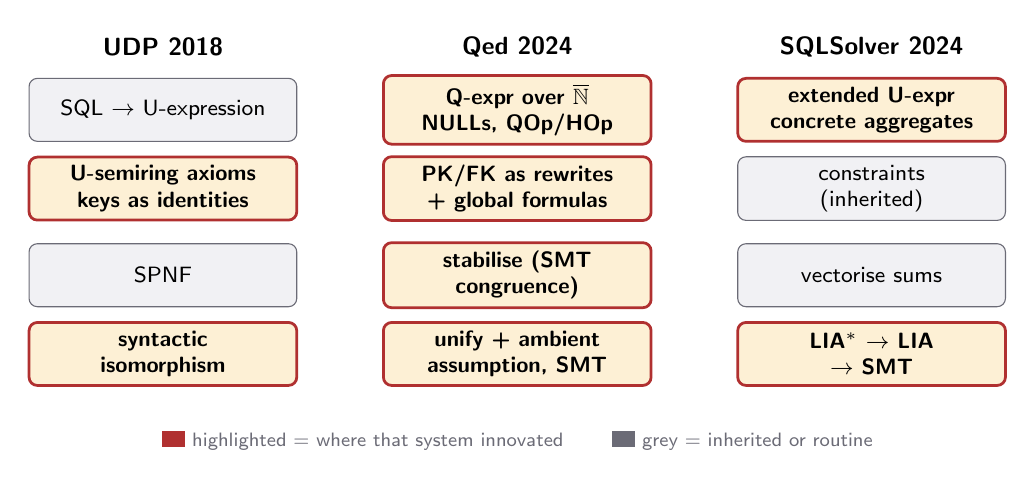
\begin{tikzpicture}[font=\footnotesize\sffamily,
  lay/.style={draw,rounded corners=3pt,minimum width=34mm,minimum height=8mm,align=center,inner sep=3pt},
  a/.style={lay,draw=cGrey,fill=cGreyBg}, h/.style={lay,draw=cRed,fill=cAmberBg,line width=1pt}]
\node[font=\small\bfseries\sffamily] at (0,3.3) {\udp{} 2018};
\node[font=\small\bfseries\sffamily] at (4.5,3.3) {\QED{} 2024};
\node[font=\small\bfseries\sffamily] at (9,3.3) {\sqlsolver{} 2024};
\foreach \x/\t in {0/{}, 4.5/{}, 9/{}} {}
% UDP column
\node[a] at (0,2.5) {SQL $\to$ U-expression};
\node[h] at (0,1.5) {\textbf{U-semiring axioms}\\\textbf{keys as identities}};
\node[a] at (0,0.4) {SPNF};
\node[h] at (0,-0.6) {\textbf{syntactic}\\\textbf{isomorphism}};
% QED column
\node[h] at (4.5,2.5) {\textbf{Q-expr over $\Nbar$}\\\textbf{NULLs, QOp/HOp}};
\node[h] at (4.5,1.5) {\textbf{PK/FK as rewrites}\\\textbf{+ global formulas}};
\node[h] at (4.5,0.4) {\textbf{stabilise (SMT}\\\textbf{congruence)}};
\node[h] at (4.5,-0.6) {\textbf{unify + ambient}\\\textbf{assumption, SMT}};
% SQLSolver column
\node[h] at (9,2.5) {\textbf{extended U-expr}\\\textbf{concrete aggregates}};
\node[a] at (9,1.5) {constraints\\(inherited)};
\node[a] at (9,0.4) {vectorise sums};
\node[h] at (9,-0.6) {\textbf{\liastar{} $\to$ \lia{}}\\\textbf{$\to$ SMT}};
\node[align=left,font=\scriptsize\sffamily,text=cGrey] at (4.5,-1.7)
  {\textcolor{cRed}{\rule{3mm}{2mm}} highlighted = where that system innovated \qquad
   \textcolor{cGrey}{\rule{3mm}{2mm}} grey = inherited or routine};
\end{tikzpicture}
\end{center}

\noindent The picture says it: \QED{} rebuilt the \emph{modelling} and the \emph{search};
\sqlsolver{} rebuilt the \emph{translation of aggregates} and the \emph{arithmetic backend}.
They are close to orthogonal.

\subsection{Capability matrix}

\begin{table}[h]\centering\small
\begin{tabular}{@{}lccc@{}}
\toprule
 & \udp{} & \QED{} & \sqlsolver{} \\
\midrule
semantic domain & any U-semiring & $\Nbar$ only & any U-semiring\\
predicate reasoning & congruence closure & SMT & SMT\\
NULL / 3-valued logic & \textcolor{cRed}{no} & \textcolor{cGreen}{full} & partial (from \wetune{})\\
outer joins & \textcolor{cRed}{no} & \textcolor{cGreen}{yes} & partial\\
primary / foreign keys & \textcolor{cGreen}{identities} & \textcolor{cGreen}{rewrite + global formula} & inherited\\
FK cycles terminate & \textcolor{cRed}{no} & \textcolor{cGreen}{yes (lazy)} & --\\
aggregates & uninterpreted & uninterpreted ($\hop$) & \textcolor{cGreen}{concrete}\\
unknown operators & \textcolor{cRed}{unsupported} & \textcolor{cGreen}{$\qop$/$\hop$ first class} & \textcolor{cRed}{unsupported}\\
differing \#summations & \textcolor{cRed}{no} & only inside $\mathcal F_T$ & \textcolor{cGreen}{yes (\liastar{})}\\
\lstinline|ORDER BY| & \textcolor{cRed}{no} & \textcolor{cRed}{no} & \textcolor{cGreen}{yes (separate layer)}\\
bag \lstinline|INTERSECT ALL| & \textcolor{cRed}{no} & \textcolor{cRed}{no (needs monus)} & \textcolor{cGreen}{yes}\\
completeness fragment & UCQ (set \emph{or} bag) & $\mathcal F_T$ (UCQ + any theory $T$) & CQ/UCQ + a group-by fragment\\
refutation & \textcolor{cRed}{no} & \textcolor{cRed}{no} & \textcolor{cRed}{no}\\
\bottomrule
\end{tabular}
\end{table}

\subsection{A gallery of separating examples}

The fastest way to understand three provers is to see what each one alone can do.

\paragraph{(1) Syntactically different but equal predicates.}
\lstinline|WHERE a+b = 0| versus \lstinline|WHERE a = -b|.
\udp{} \textcolor{cRed}{fails} --- congruence closure treats $+$ as uninterpreted.
\QED{} and \sqlsolver{} \textcolor{cGreen}{succeed} --- both call an SMT solver on
predicates. This single limitation is why \emph{everyone} after 2018 uses SMT.

\paragraph{(2) Aggregate pushdown through a key join} (\S\ref{sec:running}).
Needs: primary key as an algebraic fact \emph{and} context-sensitive comparison of the two
aggregate arguments. \QED{} \textcolor{cGreen}{succeeds} via
$S\rightsquigarrow\lam{a}{\sq{S(a)}}$ plus the $\phi_1\vee\phi_2$ ambient assumption.
\udp{} \textcolor{cRed}{fails} on the context-free recursive check (\S\ref{sec:udp-fails}).
\spes{} \textcolor{cRed}{fails} --- no applicable key rule.

\paragraph{(3) Differing numbers of summations} (Example~\ref{ex:splitunion}).
\sqlsolver{} \textcolor{cGreen}{succeeds} via \liastar{}.
\udp{} \textcolor{cRed}{fails} at Alg.~2 line 3 (term counts differ).
\QED{} \textcolor{cGreen}{also succeeds} here --- but only because this query lies in
$\mathcal F_T$, so the \emph{complete-fragment} algorithm applies: Alg.~3 groups terms by
relational scope and compares $\ind{P_1}+\cdots+\ind{P_n}$ against
$\ind{P'_1}+\cdots+\ind{P'_m}$ with $n\neq m$ allowed. This exact pattern is the paper's own
motivating example for that step.
\emph{Outside} $\mathcal F_T$ --- i.e.\ as soon as a \texttt{GroupBy}, \texttt{Distinct},
\texttt{Minus} or unknown operator appears --- \QED{} falls back to Alg.~6, which needs a
\textbf{bijection} between terms and returns \textsc{Unknown} when the counts differ. And
neither \QED{} algorithm relates sums with \emph{different relational scopes}; \liastar{}
does, and it applies uniformly rather than only inside a fragment.

\paragraph{(4) A sum of counts equals a count.}
\begin{lstlisting}[style=sql]
Q1: select a, count(b) from R group by a
Q2: select S.a, sum(S.cnt)
    from (select a, count(b) as cnt from R group by a) S group by S.a
\end{lstlisting}
\sqlsolver{} \textcolor{cGreen}{succeeds} --- it knows what \textsc{Sum} and \textsc{Count}
mean. \udp{} and \QED{} \textcolor{cRed}{cannot}, at any level of cleverness: with
aggregates uninterpreted, the required fact is simply not expressible. This is why
``aggregates'' is \QED{}'s largest Calcite failure bucket (96 cases).

\paragraph{(5) Redundant self-join on a unique key} (\cite{qed} \S6.3.2).
\begin{lstlisting}[style=sql]
Q1: select R.a from R join S S1 on R.a=S1.k join S S2 on R.a=S2.k
Q2: select R.a from R join S on R.a=S.k
\end{lstlisting}
\QED{} \textcolor{cGreen}{succeeds}: stabilisation finds $k_1=k_2=a$ through the SMT
congruence classes, then $\sq{S(a)}\times\sq{S(a)}=\sq{S(a)}$.
\spes{} \textcolor{cRed}{fails}: its self-join-on-key rule matches $R\bowtie(S\bowtie S)$, not
$(R\bowtie S)\bowtie S$, and it cannot infer $S_1.k=S_2.k$ transitively.
\textbf{Note this example has no top-level squash} --- the answer genuinely has multiplicity
2 --- so \QED{} discharges it by proving the summands equal \emph{pointwise}, not by turning
$\usum{}$ into $\exists$.

\paragraph{(6) Predicate pushdown through a left join} (\cite{qed} \S6.3.1).
\begin{lstlisting}[style=sql]
Q1: select * from (select * from R where R.a=42) X left join S on X.a=S.b
Q2: select * from (select * from R where R.a=42)
                  left join (select * from S where S.b=42) on TRUE
\end{lstlisting}
\QED{} \textcolor{cGreen}{succeeds}. \spes{} \textcolor{cRed}{fails}, and \QED{}'s paper
reports the reason as a soundness bug: it states that one of \spes{}'s normalisation rules
\emph{unsoundly} rewrites a left join whose condition is \texttt{TRUE} into a cross join.
(We report this as \cite{qed}'s claim; we did not reproduce it.) Anything needing NULL semantics
is out of reach for \udp{} entirely.

\paragraph{(7) \lstinline|ORDER BY| anything.} \sqlsolver{} only.

\subsection{The deep structural difference: squashed versus not}

Everything above has one root cause, and it is worth isolating because it predicts which
examples a given prover will handle.

When the top-level expression is \textbf{squashed} --- \lstinline|SELECT DISTINCT|,
\lstinline|GROUP BY|, \lstinline|EXISTS| --- multiplicities are irrelevant. \QED{} can then
push $\neq0$ inward, turning $\usum{}$ into $\exists$, $\times$ into $\wedge$ and $+$ into
$\vee$, and hand a pure Boolean formula to SMT. Cheap and strong.

When it is \textbf{not squashed} --- plain projection, a join, a \lstinline|UNION ALL| ---
the counts \emph{are} the answer, and the two systems fall back on comparing summands
pointwise, justified by
$(\forall \vec s.\ f(\vec s)=g(\vec s))\Rightarrow \usum{\vec s}f=\usum{\vec s}g$. That is
sound but demands \emph{alignable scopes}: \udp{}'s Alg.~2 and \QED{}'s Alg.~6 both require a
one-to-one match between terms. (\QED{}'s Alg.~3 relaxes this to ``same relational scope'',
which is strictly weaker but only available inside $\mathcal F_T$.)
\sqlsolver{} instead reasons about the sums' \emph{values}, which needs no alignment at all.

\keybox{Why the squash matters in practice}{%
Under a squash the comparison is Boolean, so a \lstinline|UNION ALL| split like
Example~\ref{ex:splitunion} reduces to
$\exists y.(y{\le}1000\wedge R{\neq}0)\vee\exists y.(y{>}1000\wedge z{<}500\wedge R{\neq}0)
\leftrightarrow \exists y.(\ldots)$ --- an ordinary SMT query that any SMT-backed tool settles.
Without the squash the same rewrite is an \emph{arithmetic} statement about sums. \QED{}
can still discharge it \emph{if} the terms share a relational scope and the query is in
$\mathcal F_T$ (Alg.~3 sums the bodies); otherwise it needs a term bijection.
\liastar{} needs neither condition.}

\subsection{On the published numbers}

\begin{table}[h]\centering\small
\begin{tabular}{@{}llrr@{}}
\toprule
reported by & benchmark described as & \spes{} & the paper's own tool\\
\midrule
\QED{}~\cite{qed}       & ``232 Calcite pairs'' & \textbf{95} & 147\\
\sqlsolver{}~\cite{sqlsolver} & ``232 Calcite pairs'' & \textbf{99} & 232\\
\bottomrule
\end{tabular}
\end{table}

\noindent The same baseline on nominally the same benchmark differs. The extraction
pipelines are different, so the suites are different, so the percentages are not
comparable. Additional cautions:

\begin{itemize}
\item \QED{}'s harder suites (444 non-trivial Calcite v1.32 pairs; 1287 CockroachDB pairs)
      were never run through \sqlsolver{}, and vice versa.
\item \QED{} does not evaluate against \sqlsolver{} at all --- the two are near-simultaneous.
\item \sqlsolver{}'s TPC-C/TPC-H pairs were generated by running Spark SQL's optimiser and
      then \emph{manually} converting logical plans back into SQL. That is a reasonable
      methodology but it is not an independent benchmark.
\item ``Proves 100\% of Calcite'' should be read as ``100\% of the pairs this group
      extracted and chose to model''.
\end{itemize}

\warnbox{If you are writing a paper in this area}{%
Do not cite a cross-paper number as a head-to-head comparison. The only defensible
comparison is one you run yourself, on one extraction, with all tools on the same input.
As of these two papers, nobody has done that.}

\subsection{What the combination would look like}

The two 2024 systems are complementary to an unusual degree, and the merge is not
speculative --- each piece has a clean interface.

\begin{center}
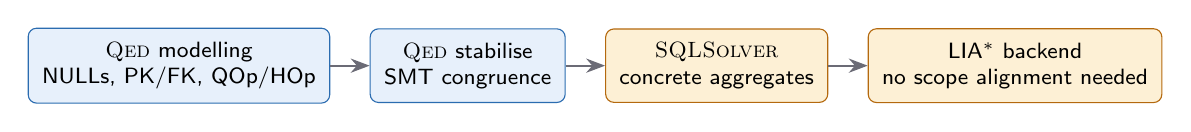
\begin{tikzpicture}[font=\footnotesize\sffamily,node distance=5mm,
  b/.style={draw=cGrey,fill=cGreyBg,rounded corners=3pt,inner sep=5pt,align=center,minimum height=9mm},
  q/.style={draw=cBlue,fill=cBlueBg,rounded corners=3pt,inner sep=5pt,align=center,minimum height=9mm},
  s/.style={draw=cAmber,fill=cAmberBg,rounded corners=3pt,inner sep=5pt,align=center,minimum height=9mm},
  ar/.style={-{Stealth[length=2.4mm]},cGrey,thick}]
\node[q] (m) {\QED{} modelling\\NULLs, PK/FK, QOp/HOp};
\node[q,right=of m] (st) {\QED{} stabilise\\SMT congruence};
\node[s,right=of st] (ag) {\sqlsolver{}\\concrete aggregates};
\node[s,right=of ag] (li) {\liastar{} backend\\no scope alignment needed};
\draw[ar](m)--(st);\draw[ar](st)--(ag);\draw[ar](ag)--(li);
\end{tikzpicture}
\end{center}

\QED{}'s term-bijection step is its ceiling; \liastar{} is exactly the tool that removes
that ceiling. \QED{}'s uninterpreted $\hop$ for aggregates is its largest failure bucket;
\sqlsolver{}'s aggregate tables fill it. Conversely \sqlsolver{}'s weakest areas --- NULLs,
constraints, unknown operators --- are precisely \QED{}'s contributions. No published system
does this.

\section{An implementer's guide}
\label{sec:impl}

This section is the advice we wish the papers had included. It assumes you are building on
Calcite (all of \spes{}, \QED{} and \sqlsolver{} consume relational plans, and Calcite's
\texttt{RelNode} is the easiest source).

\subsection{Build order}

Do not start with the fancy parts. In dependency order:

\begin{enumerate}
\item \textbf{Plan $\to$ algebra.} Handle \texttt{TableScan}, \texttt{Filter},
      \texttt{Project}, \texttt{Join}, \texttt{Union(all=true)} only. Represent an expression
      as a sum of terms; a term as (scope, body predicate, list of table applications).
\item \textbf{Normalisation to sum-of-products.} Pure syntax; no solver needed. Test by
      round-tripping and by evaluating both forms on small random instances.
\item \textbf{Pointwise term matching} with scope permutation. At this point you can already
      prove filter/projection/join reordering.
\item \textbf{Bring in SMT for predicates.} This is the single biggest capability jump per
      line of code --- it is the whole difference between \udp{} and its successors.
\item \textbf{Stabilisation} via congruence classes. Second biggest jump.
\item \textbf{Primary keys.} One rewrite. Suddenly a large class of real rules becomes
      provable.
\item \textbf{Squash/\texttt{Distinct}/\texttt{GroupBy}}, then the $\neq0$ Boolean encoding.
\item Only then: NULLs, foreign keys, uninterpreted operators, \liastar{}.
\end{enumerate}

\subsection{Data structures}

\begin{lstlisting}[style=pseudo]
Term   = { scope : List<(TableSym, Var, int power)>,   # Sum over R^k(s)
           body  : Formula,                            # the [P] part, SMT-encodable
           value : Expr }                              # the V part (QOp/HOp applications)
Expr   = List<Term>                                    # a sum of terms
\end{lstlisting}

Keep \texttt{body} in your SMT library's AST from the very beginning. Converting a
home-grown predicate type into SMT later is a rewrite you will do twice.

\subsection{Ten traps, each of which will cost you a day}

\begin{enumerate}
\item \textbf{\lstinline|GROUP BY| needs a squash.} \udp{}'s printed de-sugaring
      (Remark~\ref{rem:groupby}) iterates over every row of $R$, not every distinct key. Use
      \QED{}'s two-factor rule: $\sq{\usum{s}\ind{x=k(s)}Q(s)}\times\ind{y=\alpha(\ldots)}$.
      Get this wrong and multiplicities are silently wrong for duplicated keys.

\item \textbf{The primary-key rule for tables with non-key columns.} Eq.~\eqref{eq:pk8},
      $R\rightsquigarrow\lam{k}{\sq{R(k)}}$, applies only when the key is the \emph{whole}
      schema. In general use Eq.~\eqref{eq:pk7} with the functional-dependency symbol $f_R$.
      Almost every write-up quotes the easy form.

\item \textbf{Foreign-key chasing may not terminate.} \udp{} says so explicitly: a cycle in
      the FK graph loops. Either bound the depth or do what \QED{} does --- emit
      $\forall b,k.\ \sq{S(b,k)}\to\sq{R'(k)}$ as one global assertion and let the solver
      unfold it lazily.

\item \textbf{Over-approximation is one-directional.} In \sqlsolver{}'s non-linear path,
      \textsc{unsat} means equivalent, \textsc{sat} means \emph{nothing}. If you report
      ``not equivalent'' on \textsc{sat} you have an unsound tool.

\item \textbf{Permutation blowup.} $\textsf{termEq}$ enumerates bijections between scopes;
      \QED{} caps at 24 and reports $\sim$98\% of cases match on the identity permutation.
      Try identity first, always.

\item \textbf{Linearisation blowup.} $\mathrm{Lin}(X)$ is the ordered Bell number:
      $1,1,3,13,75,541,4683$. Eager linearisation on a term with five variables already
      generates 541 cases \emph{per table}. Use it only inside the complete fragment.

\item \textbf{Congruence classes only find expressions already present.} Given
      $\ind{x+3=10}$ they will not produce $x=7$. If you need that, call SyGuS.

\item \textbf{Finiteness.} \QED{} assumes every table has finite multiplicity at each row so
      that $\infty$ never appears during term comparison. If you model tables as
      $S\to\Nbar$ you must handle $\infty$ arithmetic; if as $S\to\mathbb{N}$ you must not
      claim completeness over all U-semirings.

\item \textbf{Bag \lstinline|EXCEPT ALL| / \lstinline|INTERSECT ALL| are not free.} They need
      truncated subtraction (monus). \QED{} declines and treats them as unknown operators;
      \sqlsolver{} encodes \lstinline|INTERSECT ALL| as
      $\ind{f_l\le f_r}f_l+\notu{\ind{f_l\le f_r}}f_r$, the pointwise minimum. Pick one
      deliberately.

\item \textbf{Implicit casts.} \QED{}'s failure table lists ``typing'' for 6 Calcite and 26
      CockroachDB pairs. Calcite inserts \texttt{CAST} nodes freely; if you model casts as
      uninterpreted functions, two plans that differ only in an implicit cast will not
      unify. Decide early whether to erase casts (unsound in general) or model them.
\end{enumerate}

\subsection{Testing: use a real database}

The cheapest high-value test harness is differential testing against PostgreSQL, and it
catches translation bugs that no amount of staring will.

\begin{lstlisting}[style=pseudo]
for each candidate rewrite (Q1, Q2):
    1. generate small random instances (0-5 rows, heavy duplicates, some NULLs)
    2. run both queries in Postgres, compare as BAGS:
         (Q1 EXCEPT ALL Q2) must be empty  AND  (Q2 EXCEPT ALL Q1) must be empty
    3. if they differ  -> your prover must NOT say "equivalent"
    4. also evaluate your U-/Q-expression directly on the same instance
       and check it reproduces Postgres' multiplicities row by row
\end{lstlisting}

Step 4 is the one people skip and the one that matters: it validates the \emph{translation},
independently of the decision procedure. Two specific settings to include:

\begin{itemize}
\item \textbf{duplicates in the right-hand table of every join} --- this is what separates a
      correct key model from a wrong one. Our running example produces $(1,60)$ versus two
      copies of $(1,30)$ (\S\ref{sec:pkcounter}); if your translation does not reproduce
      exactly that, your \texttt{GroupBy} or key rule is wrong.
\item \textbf{\lstinline|NULL| in every nullable column} --- three-valued \texttt{AND}/\texttt{OR}
      is easy to get subtly wrong, and \textsf{Null} \texttt{And} \textsf{False} $=$
      \textsf{False} is the canonical check.
\end{itemize}

Use a session-local table to shadow a real one when you want a no-key variant, so you never
mutate the reference schema:

\begin{lstlisting}[style=sql]
create temp table s (a int, b int);        -- hides the real s, no primary key
insert into s values (1,100),(1,100);
\end{lstlisting}

\subsection{Getting plans out of Calcite}

For the record, this is all it takes to obtain the trees in \S\ref{sec:running}:

\begin{lstlisting}[style=pseudo]
SchemaPlus root = Frameworks.createRootSchema(true);
root.add("R", tableOf("X","Y", /*rows*/1e6, /*key*/null));
root.add("S", tableOf("A","B", /*rows*/5e4, /*key*/0));   // column 0 unique
FrameworkConfig cfg = Frameworks.newConfigBuilder().defaultSchema(root).build();
Planner p = Frameworks.getPlanner(cfg);
RelNode rel = p.rel(p.validate(p.parse(sql))).rel;
System.out.println(RelOptUtil.toString(rel, SqlExplainLevel.EXPPLAN_ATTRIBUTES));
\end{lstlisting}

Declare uniqueness through the table's \texttt{Statistic}:
\lstinline[style=pseudo]|Statistics.of(rows, ImmutableList.of(ImmutableBitSet.of(0)))|.
That one bit is what makes Calcite's \texttt{AggregateJoinTransposeRule} produce $Q_2$
instead of the compensated \texttt{SUM $\times$ COUNT} plan of \S\ref{sec:calcite-fires} ---
and it is the same bit your prover needs for the key rewrite. A \texttt{Planner} instance is
single-use; build a fresh one per query.

\appendix
\section{All axioms and definitions on one page}
\label{app:axioms}

\subsection*{U-semiring (\udp{}) --- the complete axiom set}

\noindent$(\Usemi,0,1,+,\times)$ is a commutative semiring:
associativity and commutativity of $+$ and $\times$; $0$ is the unit of $+$; $1$ of
$\times$; $\times$ distributes over $+$; $0\times x=0$.

\begin{center}
\begin{tabular}{@{}ll@{\qquad}ll@{}}
\toprule
\multicolumn{2}{@{}l}{\textbf{squash}} & \multicolumn{2}{l}{\textbf{negation}}\\
$\sq{0}=0$ & $\sq{1+x}=1$ & \multicolumn{2}{l}{$\notu{0}=1$}\\
\multicolumn{2}{@{}l}{$\sq{\sq{x}+y}=\sq{x+y}$} & \multicolumn{2}{l}{$\notu{x\times y}=\sq{\notu{x}+\notu{y}}$}\\
\multicolumn{2}{@{}l}{$\sq{x}\times\sq{y}=\sq{x\times y}$} & \multicolumn{2}{l}{$\notu{x+y}=\notu{x}\times\notu{y}$}\\
\multicolumn{2}{@{}l}{$\sq{x}\times\sq{x}=\sq{x}$} & \multicolumn{2}{l}{$\notu{\sq{x}}=\sq{\notu{x}}=\notu{x}$}\\
\multicolumn{2}{@{}l}{$x\times\sq{x}=x$} & &\\
\multicolumn{2}{@{}l}{$x^2=x\;\Rightarrow\;\sq{x}=x$} & &\\
\midrule
\multicolumn{2}{@{}l}{\textbf{unbounded summation}} & \multicolumn{2}{l}{\textbf{predicates \& equality}}\\
\multicolumn{2}{@{}l}{$\usum{t}(f_1+f_2)=\usum{t}f_1+\usum{t}f_2$} & \multicolumn{2}{l}{$\ind{b}=\sq{\ind{b}}$}\\
\multicolumn{2}{@{}l}{$\usum{t_1}\usum{t_2}f=\usum{t_2}\usum{t_1}f$} & \multicolumn{2}{l}{$\ind{e_1{=}e_2}+\ind{e_1{\neq}e_2}=1$}\\
\multicolumn{2}{@{}l}{$x\times\usum{t}f=\usum{t}(x\times f)$} & \multicolumn{2}{l}{$f(e_1)\ind{e_1{=}e_2}=f(e_2)\ind{e_1{=}e_2}$}\\
\multicolumn{2}{@{}l}{$\sq{\usum{t}f(t)}=\sq{\usum{t}\sq{f(t)}}$} & \multicolumn{2}{l}{$\usum{t}\ind{t{=}e}=1$}\\
\midrule
\multicolumn{4}{@{}l}{\textbf{derived:}\quad $\usum{t}\ind{t{=}e}\times f(t)=f(e)$
\qquad \textbf{(Lemma \ref{lem:15} --- the workhorse)}}\\
\midrule
\multicolumn{4}{@{}l}{\textbf{KEY} $R.k$:\quad $\ind{t.k{=}t'.k}\times R(t)\times R(t')=\ind{t{=}t'}\times R(t)$}\\
\multicolumn{4}{@{}l}{\textbf{FOREIGN KEY} $S.k'\to R.k$:\quad $S(t')=S(t')\times\usum{t}R(t)\times\ind{t.k{=}t'.k'}$}\\
\bottomrule
\end{tabular}
\end{center}

\subsection*{Q-expressions (\QED{}) --- definitions, not axioms}

\noindent Domain $\Nbar=\mathbb{N}\cup\{\infty\}$ with
$\infty+a=\infty$, $0\times\infty=0$, $a\times\infty=\infty$ for $a\neq0$.
\[
\usum{s}f(s)=\begin{cases}f(s_1)+\cdots+f(s_n)&\mathrm{supp}(f)=\{s_1..s_n\}\text{ finite}\\ \infty&\text{else}\end{cases}
\qquad
\ind{P}=\begin{cases}1&P\\0&\neg P\end{cases}
\qquad
\sq{a}=\ind{a\neq0}
\qquad
\notu{a}=\ind{a=0}
\]

\begin{center}
\begin{tabular}{@{}ll@{}}
\toprule
\textbf{primary key} (general) & $R\rightsquigarrow\lam{k,s}{\sq{R'(k)}\times\ind{s=f_R(k)}}$\\
\textbf{primary key} (key = whole schema) & $R\rightsquigarrow\lam{k}{\sq{R(k)}}$\\
\textbf{foreign key} & $\forall b,k.\ \sq{S(b,k)}\to\sq{R'(k)}$ (global assertion)\\
\textbf{check} $C$ & $\forall s.\ \sq{R(s)}\to C(s)$\\
\midrule
\textbf{$\neq0$ encoding} & $\usum{s}U\rightsquigarrow\exists s.U$; \;
$U_1{\times}U_2\rightsquigarrow U_1\wedge U_2$; \;
$U_1{+}U_2\rightsquigarrow U_1\vee U_2$;\\
& $\sq{U}\rightsquigarrow U$; \; $\ind{P}\rightsquigarrow P$\\
\midrule
\textbf{ambient assumption} & recursive checks run under $\Phi\wedge(L'_1\vee L'_2)$\\
\bottomrule
\end{tabular}
\end{center}

\subsection*{\liastar{} (\sqlsolver{})}

\[
S^*=\Bigl\{\vec v \;\Bigm|\; \vec v=\sum_{i=1}^{n}\lambda_i\vec v_i,\ \vec v_i\in S,\ \lambda_i\ge0\Bigr\}
\qquad
\liastar{}:\ \exists\vec u,\vec v.\ F_1(\vec u,\vec v)\wedge\vec v\in\{\vec x\mid F_2(\vec x)\}^*
\]
Reduction to \lia{} (Thm.~\ref{thm:liastar}): replace the closure by
$\vec v=\sum_{i=1}^{k}\lambda_i\vec x_i\wedge\bigwedge_i F_2(\vec x_i)$, where the $\vec x_i$
are generators of $F_2$. Encoding of U-terms into \lia{}:
$\ind{b}\mapsto\mathrm{ite}(b,1,0)$, $\sq{E}\mapsto\mathrm{ite}(E{=}0,0,1)$,
$\notu{E}\mapsto\mathrm{ite}(E{=}0,1,0)$, tuple/attribute/table applications $\mapsto$ fresh
integer variables.

\section{Symbol glossary}

\begin{center}
\begin{tabularx}{\linewidth}{@{}llX@{}}
\toprule
symbol & read as & SQL\\
\midrule
$R(t)$ & multiplicity of row $t$ in $R$ & \lstinline|FROM R|\\
$\ind{P}$ & $1$ if $P$ else $0$ & \lstinline|WHERE P|\\
$\times$ & multiply multiplicities & \lstinline|JOIN|\\
$+$ & add multiplicities & \lstinline|UNION ALL|\\
$\usum{a}$ & try every $a$, add up & projection (\lstinline|COUNT(*)| when applied to a table)\\
$\sq{e}$ & clamp to $0$ or $1$ & \lstinline|DISTINCT|, \lstinline|EXISTS|, \lstinline|GROUP BY| key\\
$\notu{e}$ & $1$ iff $e=0$ & \lstinline|NOT EXISTS|\\
$\lam{y}{e}$ & anonymous function; here \emph{a bag} & the group feeding an aggregate\\
$\Sumagg(\lam{y}{f})$ & $\sum_y y\times f(y)$ & \lstinline|SUM(y)|\\
$\Sumagg(\lam{y}{\sq{f}})$ & each distinct $y$ once & \lstinline|SUM(DISTINCT y)|\\
$\usum{y}\sq{f(y)}$ & count distinct values & \lstinline|COUNT(DISTINCT y)|\\
$\qop,\hop$ & uninterpreted query / scalar operator & \lstinline|LIMIT|, \lstinline|IN|, anything unmodelled\\
$\Nbar$ & $\mathbb{N}\cup\{\infty\}$ & the multiplicity domain\\
$\Gamma\mid\Delta\mid\Phi$ & tables $\mid$ other symbols $\mid$ assumptions & the proving context\\
\bottomrule
\end{tabularx}
\end{center}

\section{Reproducing the measurements}

Calcite plans (\S\ref{sec:running}, \S\ref{sec:calcite-fires}): Calcite 1.19,
\texttt{HepPlanner} with
\texttt{AggregateProjectMergeRule} $\to$ \texttt{AggregateJoinTransposeRule.EXTENDED} $\to$
\texttt{ProjectMergeRule} $\to$ \texttt{AggregateProjectMergeRule}. The first
\texttt{AggregateProjectMergeRule} is required: without it the transpose rule does not fire,
because \texttt{sql2rel} leaves a \texttt{LogicalProject} between the aggregate and the join.

PostgreSQL measurements (Fig.~\ref{fig:pgplans}): PostgreSQL 18,
\lstinline|EXPLAIN (ANALYZE, VERBOSE, BUFFERS)|; \texttt{r} $10^6$ rows with $\sim10^5$
distinct \texttt{x}, \texttt{s} $5\cdot10^4$ rows with a primary key, both \texttt{ANALYZE}d.
Equivalence spot-checked on $2\cdot10^5$ rows with \lstinline|EXCEPT ALL| in both
directions ($0$ rows each way).


\begin{thebibliography}{9}
\bibitem{udp} Shumo Chu, Brendan Murphy, Jared Roesch, Alvin Cheung, Dan Suciu.
  \emph{Axiomatic Foundations and Algorithms for Deciding Semantic Equivalences of SQL Queries.}
  PVLDB 11(11), 2018. arXiv:1802.02229.
\bibitem{qed} Shuxian Wang, Sicheng Pan, Alvin Cheung.
  \emph{QED: A Powerful Query Equivalence Decider for SQL.} PVLDB 17(11):3602--3614, 2024.
\bibitem{sqlsolver} Haoran Ding, Zhaoguo Wang, Yicun Yang, Dexin Zhang, Zhenglin Xu,
  Haibo Chen, Ruzica Piskac, Jinyang Li.
  \emph{Proving Query Equivalence Using Linear Integer Arithmetic.}
  Proc.\ ACM Manag.\ Data 1(4), Article 227 (SIGMOD), 2023.
\bibitem{spes} Qi Zhou, Joy Arulraj, Shamkant Navathe, William Harris, Jinpeng Wu.
  \emph{SPES: A Symbolic Approach to Proving Query Equivalence Under Bag Semantics.} ICDE 2022.
\bibitem{green} Todd J. Green, Grigoris Karvounarakis, Val Tannen.
  \emph{Provenance Semirings.} PODS 2007.
\bibitem{cohen} Sara Cohen. \emph{Equivalence of Queries Combining Set and Bag-Set Semantics.}
  PODS 2006.
\bibitem{piskac} Ruzica Piskac, Viktor Kuncak.
  \emph{Decision Procedures for Multisets with Cardinality Constraints.} VMCAI 2008.
\bibitem{levatich} Maxwell Levatich, Nikolaj Bj\o{}rner, Ruzica Piskac, Sharon Shoham.
  \emph{Solving LIA$^*$ Using Approximations.} VMCAI 2020.
\bibitem{wetune} Zhaoguo Wang et al. \emph{WeTune: Automatic Discovery and Verification of
  Query Rewrite Rules.} SIGMOD 2022.
\end{thebibliography}

\end{document}
